\documentclass[twoside]{article}

% file's preambule


% connect packages
%%%%%%%%%%%%%%%%%%%%%%%%%%%%%%%%%%%%%%%%%%%%%%%%%%%%%%%%%%%%%%%%%%%%%%
\usepackage[T2A]{fontenc}                   %!? закрепляет внутреннюю кодировку LaTeX
\usepackage[utf8]{inputenc}                 %!  закрепляет кодировку utf8
\usepackage[english,russian]{babel}         %!  подключает русский и английский
\usepackage{amsmath}                        %!  |
\usepackage{amssymb,textcomp, esvect,esint} %!  |важно для формул 
\usepackage[margin=2cm]{geometry}           %!  фиксирует оступ на 2cm
\usepackage{amsfonts}                       %!  математические шрифты
\usepackage{amsthm}                         %!  newtheorem и их сквозная нумерация
\usepackage{graphicx}                       %?  графическое изменение текста
\usepackage{indentfirst}                    %   добавить indent перед первым параграфом
\usepackage{xcolor}                         %   добавляет цвета
\usepackage{enumitem}                       %!  задание макета перечня.
\usepackage[unicode, pdftex]{hyperref}      %!  оглавление для панели навигации по PDF-документу + гиперссылки
\usepackage{booktabs}                       %!  добавляет книжные линии в таблицы
\usepackage{hypcap}                         %?  адресация на картинку, а не на подпись к ней
\usepackage{abraces}                        %?  фигурные скобки сверху или снизу текста
\usepackage{caption}                        %-  позволяет корректировать caption 
\usepackage{multirow}                       %   объединение ячеек в таблицах
\usepackage{pifont}                         %!  нужен для крестика
\usepackage{cancel}                         %!  аутентичное перечеркивание текста
\usepackage{ulem}                           %!  перечеркивание текста
\usepackage{tikz}                           %!  высокоуровневые рисунки (кружочек)
\usepackage{titling}                        %-  автоматическое заглавие 
\usepackage{blindtext}                      %-  слепой текст
\usepackage{fancyhdr}                       %   добавить верхний и нижний колонтитул

\usepackage{import}
\usepackage{xifthen}
\usepackage{pdfpages}
\usepackage{transparent}

\usepackage{mathrsfs}  
%%%%%%%%%%%%%%%%%%%%%%%%%%%%%%%%%%%%%%%%%%%%%%%%%%%%%%%%%%%%%%%%%%%%%%

%%%%%%%%%%%%%%%%%%%%%%% ИНТЕГРАЛЫ %%%%%%%%%%%%%%%%%%%%%%%%%%%%%%%%%%%%
\makeatletter
\def\upintkern@{\mkern-7mu\mathchoice{\mkern-3.5mu}{}{}{}}
\def\upintdots@{\mathchoice{\mkern-4mu\@cdots\mkern-4mu}%
 {{\cdotp}\mkern1.5mu{\cdotp}\mkern1.5mu{\cdotp}}%
 {{\cdotp}\mkern1mu{\cdotp}\mkern1mu{\cdotp}}%
 {{\cdotp}\mkern1mu{\cdotp}\mkern1mu{\cdotp}}}
\newcommand{\upiint}{\DOTSI\protect\UpMultiIntegral{2}}
\newcommand{\upiiint}{\DOTSI\protect\UpMultiIntegral{3}}
\newcommand{\upiiiint}{\DOTSI\protect\UpMultiIntegral{4}}
\newcommand{\upidotsint}{\DOTSI\protect\UpMultiIntegral{0}}
\newcommand{\UpMultiIntegral}[1]{%
  \edef\ints@c{\noexpand\upintop
    \ifnum#1=\z@\noexpand\upintdots@\else\noexpand\upintkern@\fi
    \ifnum#1>\tw@\noexpand\upintop\noexpand\upintkern@\fi
    \ifnum#1>\thr@@\noexpand\upintop\noexpand\upintkern@\fi
    \noexpand\upintop
    \noexpand\ilimits@
  }%
  \futurelet\@let@token\ints@a
}
\makeatother

\DeclareFontFamily{OMX}{mdbch}{}
\DeclareFontShape{OMX}{mdbch}{m}{n}{ <->s * [0.8]  mdbchr7v }{}
\DeclareFontShape{OMX}{mdbch}{b}{n}{ <->s * [0.8]  mdbchb7v }{}
\DeclareFontShape{OMX}{mdbch}{bx}{n}{<->ssub * mdbch/b/n}{}

\DeclareSymbolFont{uplargesymbols}{OMX}{mdbch}{m}{n}
\SetSymbolFont{uplargesymbols}{bold}{OMX}{mdbch}{b}{n}
\DeclareMathSymbol{\upintop}{\mathop}{uplargesymbols}{82}
\DeclareMathSymbol{\upointop}{\mathop}{uplargesymbols}{"49}

\DeclareFontEncoding{MDB}{}{}
\DeclareFontFamily{MDB}{mdbch}{}
\DeclareFontShape{MDB}{mdbch}{m}{n}{ <->s * [0.8]  mdbchrmb }{}
\DeclareFontShape{MDB}{mdbch}{b}{n}{ <->s * [0.8]  mdbchbmb }{}
\DeclareFontShape{MDB}{mdbch}{bx}{n}{<->ssub * mdbch/b/n}{}
\DeclareFontSubstitution{MDB}{cmr}{m}{n}
\DeclareSymbolFont{mathdesignB}{MDB}{mdbch}{m}{n}%
\SetSymbolFont{mathdesignB}{bold}{MDB}{mdbch}{b}{n}%
\DeclareMathSymbol{\upintclockwise}{\mathop}{mathdesignB}{128}
\DeclareMathSymbol{\upointclockwise}{\mathop}{mathdesignB}{130}
\DeclareMathSymbol{\upointctrclockwise}{\mathop}{mathdesignB}{132}
\DeclareMathSymbol{\upoiint}{\mathop}{mathdesignB}{134}
\DeclareMathSymbol{\upoiiint}{\mathop}{mathdesignB}{136}

\makeatletter
\newcommand{\upint}{\DOTSI\upintop\ilimits@}
\newcommand{\upoint}{\DOTSI\upointop\ilimits@}
\makeatother

%%%%%%%%%%%%%%%%%%%%%%%%%%%%%%%%%%%%%%%%%%%%%%%%%%%%%%%%%%%%%%%%%%%%%%



% add (renew) commands
%%%%%%%%%%%%%%%%%%%%%%%%%%%%%%%%%%%%%%%%%%%%%%%%%%%%%%%%%%%%%%%%%%%%%%
\renewcommand{\Im}{\mathop{\mathrm{Im}}\nolimits}
\renewcommand{\Re}{\mathop{\mathrm{Re}}\nolimits}
\renewcommand{\div}{\mathop{\mathrm{div}}\nolimits}
\renewcommand{\d}{\, d}
\renewcommand{\leq}{\leqslant}
\renewcommand{\geq}{\geqslant}

\newcommand{\vc}[1]{\mbox{\boldmath $#1$}}
\newcommand{\T}{^{\text{T}}}

\newcommand{\grad}{\mathop{\mathrm{grad}}\nolimits}
\newcommand{\rot}{\mathop{\mathrm{rot}}\nolimits}
\newcommand{\diag}{\mathop{\mathrm{diag}}\nolimits}
\newcommand{\Ker}{\mathop{\mathrm{Ker}}\nolimits}
\newcommand{\Spec}{\mathop{\mathrm{Spec}}\nolimits}
\newcommand{\sign}{\mathop{\mathrm{sign}}\nolimits}
\newcommand{\tr}{\mathop{\mathrm{tr}}\nolimits}
\newcommand{\rg}{\mathop{\mathrm{rg}}\nolimits}

\newcommand{\const}{\text{const}}
\newcommand{\red}[1]{\textcolor{red}{#1}}
\newcommand{\xmark}{\ding{55}}

\renewcommand{\int}{\upint}
\renewcommand{\oint}{\upoint}
%%%%%%%%%%%%%%%%%%%%%%%%%%%%%%%%%%%%%%%%%%%%%%%%%%%%%%%%%%%%%%%%%%%%%%


% some tikz commands
%%%%%%%%%%%%%%%%%%%%%%%%%%%%%%%%%%%%%%%%%%%%%%%%%%%%%%%%%%%%%%%%%%%%%%
\makeatletter %%%%%%%%%%%%%%% КРУЖОЧЕК %%%%%%%%%%%%%%%%%%%%%%%%%%%%%%%
\newcommand*{\encircled}[1]{\relax\ifmmode\mathpalette
\@encircled@math{#1}\else\@encircled{#1}\fi}
\newcommand*{\@encircled@math}[2]{\@encircled{$\m@th#1#2$}}
\newcommand*{\@encircled}[1]{%
  \tikz[baseline,anchor=base]{\node[draw,circle,outer sep=0pt,
                                        inner sep=.2ex] {#1};}}
\makeatother

\usepackage{arydshln} %%%%%%%%%%%%%%% ЛИНИИ В МАТРИЧКЕ %%%%%%%%%%%%%%%
\makeatletter
  \renewcommand*\env@matrix[1][*\c@MaxMatrixCols c]{%
    \hskip -\arraycolsep
    \let\@ifnextchar\new@ifnextchar
  \array{#1}}
\makeatother
%%%%%%%%%%%%%%%%%%%%%%%%%%%%%%%%%%%%%%%%%%%%%%%%%%%%%%%%%%%%%%%%%%%%%%



\DeclareRobustCommand{\tmpsim}{ %%%%%%%%%%%%%% ~ < %%%%%%%%%%%%%%%%%%%
  \mathbin{\text{
      \raisebox{-1pt}{
            \hspace{-4.5pt} \rotatebox{-26}{\scalebox{0.8}[0.7]{$\sim$}}
        }
  }}
}
\def\lesim{{
    \setbox0\hbox{$\ <\ $}
    \rlap{\hbox to \wd0{\hss$\tmpsim$\hss}}\box0
}}
%%%%%%%%%%%%%%%%%%%%%%%%%%%%%%%%%%%%%%%%%%%%%%%%%%%%%%%%%%%%%%%%%%%%%%


% create environment
%%%%%%%%%%%%%%%%%%%%%%%%%%%%%%%%%%%%%%%%%%%%%%%%%%%%%%%%%%%%%%%%%%%%%%
\newtheorem{to_thr}{Thr}[section]
\newtheorem{to_suj}[to_thr]{Suj}
\newtheorem{to_lem}[to_thr]{Lem}
\newtheorem{to_law}[to_thr]{Law}
\newtheorem{to_com}[to_thr]{Com}
\newtheorem{to_con}[to_thr]{Con}
\theoremstyle{definition}
\newtheorem{to_def}[to_thr]{Def}

\newenvironment{description*}
{
    \begin{description}
        \setlength{\itemsep}{1pt}
        \setlength{\parskip}{1pt}
        }
    {\end{description}
}
%%%%%%%%%%%%%%%%%%%%%%%%%%%%%%%%%%%%%%%%%%%%%%%%%%%%%%%%%%%%%%%%%%%%%%

\newcommand{\incfig}[1]{%
    % \def\svgwidth{\columnwidth}
    \import{./figures/}{#1.pdf_tex}
}

% add some colors
%%%%%%%%%%%%%%%%%%%%%%%%%%%%%%%%%%%%%%%%%%%%%%%%%%%%%%%%%%%%%%%%%%%%%%
\definecolor{grey}{HTML}{666666}
\definecolor{linkcolor}{HTML}{0000CC}
\definecolor{urlcolor}{HTML}{006600}
\hypersetup{
    pdfstartview=FitH,  
    linkcolor=linkcolor,
    urlcolor=urlcolor, 
    colorlinks=true,
    citecolor=blue}
%%%%%%%%%%%%%%%%%%%%%%%%%%%%%%%%%%%%%%%%%%%%%%%%%%%%%%%%%%%%%%%%%%%%%%


% add page header
%%%%%%%%%%%%%%%%%%%%%%%%%%%%%%%%%%%%%%%%%%%%%%%%%%%%%%%%%%%%%%%%%%%%%%
\pagestyle{fancy}
\fancyhf{}
\fancyhead[RE,LO]{\textsc{Ф\raisebox{-1.5pt}{и}з\TeX}}
% \fancyhead[LE,RO]{ОбщеФиз}
\fancyhead[CO,CE]{\leftmark}
\fancyfoot[LE,RO]{\textcolor{grey}{\texttt{\thepage}}}
%%%%%%%%%%%%%%%%%%%%%%%%%%%%%%%%%%%%%%%%%%%%%%%%%%%%%%%%%%%%%%%%%%%%%%


\begin{document}

% set skip of equation length 

\setlength{\abovedisplayskip}{3pt}
\setlength{\abovedisplayshortskip}{3pt}
\setlength{\belowdisplayskip}{3pt}
\setlength{\belowdisplayshortskip}{3pt}

% \numberwithin{equation}{section}

% input files


\section*{Articles used}

\begin{enumerate}[label = \Roman*.]
	\item <<Dynamics of Gliding Arc Climbing
in a Unipolar Jacob’s Ladder>> by K. I. Almazov et al. 22 January 2020;

	\item <<Physical study of a gliding arc discharge>> by F. Richard et al. 20 November 1995;

	\item <<Prospects of airflow control by a gliding arc in a static magnetic field>> by N Balcon et al. 28 August 2008;

	\item <<Numerical Calculations of the Properties of Axially Symmetric Arc Columns>> by A.Wells March 1967.
\end{enumerate}
% %%%%%%%%%%%%%%%%%%%%%%%%%%%%%%%%%%%%%%%%%%%%%%%%%%%%%%%%%%%%%%%%%%%%%%%%%%%%
% \section{Principal variables and constants}
% %%%%%%%%%%%%%%%%%%%%%%%%%%%%%%%%%%%%%%%%%%%%%%%%%%%%%%%%%%%%%%%%%%%%%%%%%%%%


% The heat flux potential (потенциал теплового потока) -- 

% The Prandtl and turbulent Prandtl numbers -- 

% The eddy diffusivity for momentum (вихревой коэффициент диффузии для импульса) -- 

% The specific enthalpy (удельная энтальпия) --



%%%%%%%%%%%%%%%%%%%%%%%%%%%%%%%%%%%%%%%%%%%%%%%%%%%%%%%%%%%%%%%%%%%%%%%%%%%%
\section{Principal equations (I article)}
%%%%%%%%%%%%%%%%%%%%%%%%%%%%%%%%%%%%%%%%%%%%%%%%%%%%%%%%%%%%%%%%%%%%%%%%%%%%


\subsection{Hand waving}

I would like to write the energy equation: the rate of change of energy per unit volume. To do this, we look at heat exchange with the environment and at movement in an electromagnetic potential field.

In fact $E^2\sigma$ -- specific energy density per unit time. We also have some heat exchange with the environment.
The heat flux potential can be defined by
\begin{equation}
    S = \int_0^T \varkappa \d T,
\end{equation}
So we characterize it as $\div \grad S = \nabla^2 S$, --  specific heat exchange. Then
\begin{equation*}
    P = \sigma E^2 + \div \grad S.
\end{equation*}
We expect to see something like that.

\subsection{According to the article}


Taking into consideration only a small part of the arc, we
define a set of axes $(r,x)$ in cylindrical coordinates.
\textbf{The energy equation} for a \textbf{steady arc} is
\begin{equation}
    \rho U \frac{\partial h}{\partial x} + \rho V \frac{\partial h}{\partial r} 
    =
    \frac{1}{r} \frac{\partial }{\partial r} 
    \left[
        r \left(\frac{\mu}{P_r} + \frac{\rho \varepsilon_m}{P_{rt}} \right) 
        \frac{\partial h}{\partial r} 
    \right] + 
    \sigma E^2,
\end{equation}
and \textbf{the continuity equation} by
\begin{equation} % вроде готовы в это верить. 
    \div \vc{j}_m = \frac{1}{r} \frac{\partial }{\partial r} (r \rho V) + \frac{\partial }{\partial x} (\rho U) = 0,
\end{equation}
where $\rho$ is the density, $U$ the axial velocity, $V$ the radial velocity, $h$ the specific enthalpy, $\mu$ the viscosity, $\varepsilon_m$ the eddy diffusivity for momentum, $P_\text{t}$ and $P_\text{rt}$ the Prandtl and turbulent Prandtl numbers, respectively, $\sigma$ the electrical conductivity, and $E$ the voltage gradient.

The heat flux potential can be defined by
\begin{equation*}
    S_{(T)} = \int_0^T \varkappa_{(T)} \d T,
\end{equation*}
so that the \textbf{molecular diffusion term}
\begin{equation*}
    \frac{1}{r} \frac{\partial }{\partial r} \left[
        r \left(\frac{\mu}{P_r} \right) \frac{\partial h}{\partial r} 
    \right] \equiv \nabla^2 S
\end{equation*}
in the energy equation can be replaced.


%%%%%%%%%%%%%%%%%%%%%%%%%%%%%%%%%%%%%%%%%%%%%%%%%%%%%%%%%%%%%%%%%%%%%%%%%%%%
\subsection{Assumptions}
%%%%%%%%%%%%%%%%%%%%%%%%%%%%%%%%%%%%%%%%%%%%%%%%%%%%%%%%%%%%%%%%%%%%%%%%%%%%


To describe the arc, we use a simplified model in which
rough assumptions are made. These assumptions were used 
by Maecker and Frind to describe cylindrical arc behavior. 
\begin{enumerate*}
    \item Flow is axially symmetrical.
    \item Viscous dissipation and Lorentz forces can be neglected.
    \item  Radial pressure gradient is negligible compared to the
        static pressure.
    \item  Radiation is neglected.
    \item  Principal transfer of energy is produced by conduction
        and convection.
\end{enumerate*}


We consider two arc regions separately -- 
\textbf{the plasma core}, 
also called plasma string, 
and 
\textbf{the outer flame} or weak ionized ring.




%%%%%%%%%%%%%%%%%%%%%%%%%%%%%%%%%%%%%%%%%%%%%%%%%%%%%%%%%%%%%%%%%%%%%%%%%%%%
\subsection{The plasma string model}
%%%%%%%%%%%%%%%%%%%%%%%%%%%%%%%%%%%%%%%%%%%%%%%%%%%%%%%%%%%%%%%%%%%%%%%%%%%%

Based on experimental results, although the arc is moving, the plasma channel can be considered to be \textbf{in a steady state with a constant radius}. Physical properties along the center line of the plasma string are assumed to be the same at
every point on the line. As a result of the longitudinal convection affecting the arc, the form is assumed to be cylindrical.

Let us consider a small part of the plasma string which is assumed to be identical to any other section of the plasma arc.

The emission of light being the same all along the string,
we assume
\begin{equation}
    \frac{\partial h}{\partial x} = 0.
\end{equation}
Turbulent effects and radial convection can be neglected for heat exchanges
\begin{equation}
    V \frac{\partial h}{\partial r} = 0.
\end{equation}
The energy equation is rewritten
\begin{equation}
    0   =
    \frac{1}{r} \frac{\partial }{\partial r} 
    \bigg[
        r \bigg(\frac{\mu}{P_r} + 
        \underbrace{\frac{\rho \varepsilon_m}{P_{rt}}}_{0?}
        \bigg) 
        \frac{\partial h}{\partial r} 
    \bigg] + \sigma E^2,
\end{equation}
rewriting in a different form,
\begin{equation}
    \nabla^2 S + \sigma E^2 = 0,
\end{equation}
which corresponds to the well known (авторами статьи) \textbf{Elenbaas–Heller equation}.


%%%%%%%%%%%%%%%%%%%%%%%%%%%%%%%%%%%%%%%%%%%%%%%%%%%%%%%%%%%%%%%%%%%%%%%%%%%%
\subsection{The arc core-outer flame transition}
%%%%%%%%%%%%%%%%%%%%%%%%%%%%%%%%%%%%%%%%%%%%%%%%%%%%%%%%%%%%%%%%%%%%%%%%%%%%

At the boundary of the arc core and the outer flame, the temperature profile in the plasma string is assumed to be invariable with a constant conducting radius $r_c$.


Convection is, therefore, the main cause of plasma string  cooling. It constricts the arc as the difference in velocity between arc–core and the surrounding region increases. The constant plasma string radius is evidence of an equivalent
constant convection effect expressed in terms of an axially symmetrical convection flow.

The convection term does not appear in the energy balance equation of the plasma string, but is implicitly taken into account in the input value of the electric field and power per unit of length deduced from experiments. 

In the conductive inner part of the discharge, the electrical conductivity is given as a linear function of heat flux potential
\begin{equation}
    \sigma = \beta (S - S_{\text{c}}),
\end{equation}
where $S_C$ is the heat flux potential for $\sigma=0$ correspondings to the conduction radius $r_c$.

 The conduction radius is 
\begin{equation}
    \vc{r}_c \sim \frac{1}{\sqrt{\beta} E} .
\end{equation}
The power per unit of discharge length $w$ is related to $S_0$ which corresponds to the axis heat flux potential ($r=0$), on which the temperature is $T_0$, according to the following equation:
\begin{equation*}
    S_0 = \frac{w}{2\pi} + S_c.
\end{equation*}


% \newpage
\section{Staged experiment (II articls)}


Devices with a gliding arc are classified according
to power supply regime as <<\textbf{bipolar}>> and \textbf{unipolar}>>.
In the bipolar regime of power supply, sign-alternating 
sinusoidal voltage is applied to two electrodes of a
device.

In this experiment and ours, we work with a Flyback transformer, so that the signal is rectified in the unipolar case.

\begin{figure}[h]
    \centering
    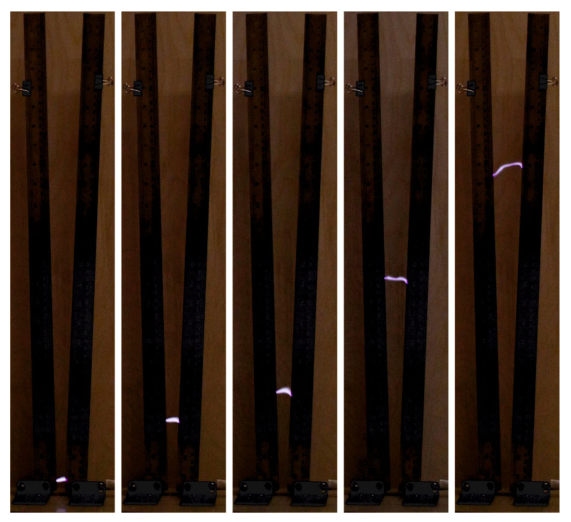
\includegraphics[width=0.3\textwidth]{figures/1.png}
    \caption{Experiment for Article II.}
\end{figure}

It was founded, that it moves with a constant velocity on most of the path. Also, the the dependence of the arc rise speed on the angle between the electrodes was investigated.


\section{Staged experiment (III articls)}


A slightly more meaningful experiment was set up in the next article, it has yet to be analyzed.

\begin{figure}[h]
    \centering
    \includegraphics[width=0.4\textwidth]{figures/2.png}
    %\caption{}
    %\label{fig:}
\end{figure}





% % document's head
% \phantom{42}

\begin{center}
    \LARGE \textsc{Заметки курса <<Электричество и магнетизм>>}
\end{center}

\hrule

\phantom{42}

\begin{flushright}
    \begin{tabular}{rr}
    % written by:
        \textbf{Автор}: 
        & Хоружий Кирилл \\
        &\\
    % date:
        \textbf{От}: &
        \textit{\today}\\
    \end{tabular}
\end{flushright}

\thispagestyle{empty}
\tableofcontents
% \newpage


% \input
% \input







\end{document} Для точки $P$ движущейся относительно некоторого неподвижного тела (свяжем с ним точку $O$), можно ввести следующие характеристики:
\begin{to_def}[Радиус вектор, скорость и ускорение точки $P$]
	\begin{equation*}
	\vc{r} = \overrightarrow{O P},
	\hspace*{1 cm}
	\vc{v} = \frac{d \vc{r}}{d \vc{t}},
	\hspace*{1 cm}
	\vc{w} =  \frac{d \vc{v}}{d t} = \frac{d^2 \vc{r}}{d t^2}.
\end{equation*}	
\end{to_def}

\begin{to_def}
	Для задания движения точки, зная её траекторию, можно сопоставить ей дуговую координату $\sigma (t)$ и получить выражения для скорости и ускорения, выраженные в осях \textit{естественного трёхгранника} $\vc{\tau}, \vc{n}, \vc{b}$.
	Таким образом для $\vc{r} = \vc{r}(\sigma(t))$:
	\begin{equation*}
		\vc{\tau} (\sigma) = \frac{d \vc{r}}{d \sigma}, 
		\hspace*{1 cm} 
		\frac{d \vc{\tau}}{d \sigma} = \frac{1}{\rho} \vc{n} (\sigma),
	\end{equation*}
	где $\rho$ -- радиус кривизны. Для кривой в $\mathbb{R}^3$ добавим ещё вектор $b$ для правой тройки. Таким образом получим формулы Френе:
	\begin{equation*}
		\frac{d \vc{\tau}}{d s} = \frac{1}{\rho} \vc{n},
		\hspace*{1 cm}
		\frac{d \vc{n}}{d s} = - \frac{1}{\rho} \vc{\tau} + \varkappa \vc{b},
		\hspace*{1 cm}
		\frac{d \vc{b}}{d s} = - \varkappa \vc{n}.
	\end{equation*}
\end{to_def}

Таким образом сможем в компонентах трёхгранника выписать скорость и ускорение точки:
\begin{gather*}
   \vc{v} = \frac{d \vc{r}}{d t} = \frac{d \vc{r}}{d \sigma} \frac{d \sigma}{d t} = v_\tau \vc{\tau}
   \\
   \vc{w} = \frac{d \vc{v}}{d t} = \frac{d_\tau}{d t} \vc{\tau} + v_\tau \frac{d \vc{\tau}}{d \sigma} \frac{d \sigma}{d t} = \frac{d^2 \sigma}{d t^2} \vc{\tau} + \frac{v_\tau^2}{\rho} \vc{n}.
\end{gather*}
Как видно, ускорение точки представилось в видео $w = w_n + w_\tau $ --- \textit{нормальной} и \textit{тангенциальной} составляющей.

\begin{to_lem}[Из матана]
	Для $f_i \in  C^2 \colon U \mapsto V$, если $X$ -- касательный вектор в точке $p \in U$, то $X(f)$ можно определить как:
	\begin{equation*}
		X(f) = X(x^i) \frac{\partial f(p)}{\partial x^i}, \text{ а координаты этого вектора в криволинейных координатах: } X = X^i \frac{\partial}{\partial x^i}.
	\end{equation*}
\end{to_lem}

Каждую материальную точку можем определить $\vc{r}_1, \ldots, \vc{r}_N$ -- итого $\mathbb{R}^{3N}$. Но есть некоторые ограничения вида
\begin{equation*}
    f_i (\vc{r}, t) = 0.
\end{equation*}
Вложим в фазовое пространство многообразие $M$, в котором локально всё хорошо. Тогда
$\dim M = n$ -- число степеней свободы, а параметризация $q_1, \ldots, q_N$ -- криволинейные координаты. В каждой $A \in M$ верно, что $\dot{\vc{q}} \in TM_A$, то есть
\begin{equation}
    TM = \bigcup_q T_qM \ni (q, \dot{q})
\end{equation}

И такБ движение точки можно задать, если её криволинейные координаты --- известне функции $q(t)$.
\begin{equation*}
	\vc{r} = \vc{r}(q_1, q_2, q_3) = x \vc{i} + y \vc{j} + z \vc{k}.
\end{equation*}

\begin{to_def}
	\textit{Коэффициентами Ламе} такие $H^i$. C их помощью удобно выразить единичные базисные векторы криволинейных координат: 
	\begin{equation*}
		H_i = \left|\frac{\partial \vc{r}}{\partial q^i} \right| = \sqrt{\left(\frac{\partial x}{\partial q^i}\right)^2 + \left(\frac{\partial y}{\partial q^i}\right)^2 + \left(\frac{\partial z}{\partial q^i}\right)^2}.
		\hspace*{1 cm}
		e^i = \frac{1}{H_i} \frac{\partial \vc{r}}{\partial q^i}.
	\end{equation*}
\end{to_def}

Далее будем координатными векторами называть $\vc{g}_i(\vc{r}) = \frac{\partial \vc{r}}{\partial q^i}$. Разложение произвольного вектора по локальному базису имеет вид:
\begin{equation*}
	\vc{a} = a^i \vc{g}_i = a_j \vc{g}^j.
\end{equation*}
Здесь $\vc{g}^j$ --- векторы двойственного базиса к базису из $\vc{g}_i$. В двойственном же (взаимном) базисе из матана мы видели:
\begin{equation*}
	X(f) = d f (X) = \partial_x f,
	\hspace*{1 cm}
	d x^i (\frac{\partial}{\partial x^j}) = \frac{\partial x^i}{\partial x^j} = \delta_j^i,
	\hspace*{1 cm}
	a = a_i d x^i.
\end{equation*}
Таким образом получаем скорость точки и её ковариантную компоненту:
\begin{equation*}
	\vc{v} = \frac{d \vc{r}}{d t} = \frac{\partial \vc{r}}{\partial q^i} \frac{d q^i}{d t} = \vc{g}_i \dot{q}^i,
	\hspace*{1 cm}
	v^i = \vc{q}^i.
\end{equation*}
И для ускорения:
\begin{equation*}
	w_k = \left(\frac{d \vc{v}}{d t}\right)_k = \frac{(d \vc{v})_k}{d t} = g_{k j} \frac{d v^j}{d t} + \Gamma_{k i j} v^j v^i.
\end{equation*}
\begin{to_def}
	\textit{Твёрдое телое} --- множество точек, расстояние между которыми не меняется: $\forall j, j, t \colon \vc{|r}_i(t) - \vc{r}_j| = \const$. 
\end{to_def}

Точка $O$ это полюс. Во-первых перенесем начало координат в $O$. Введём систему координат $O_{\xi\nu\zeta}$ связанную с телом, -- тело относительно неё не движется
\begin{equation*}
	 \vc{r} = \vv{OA}, \, \vc{\rho} = \vv{OA} = \const \text{ в $O_{\xi\nu\zeta}$},
    \hspace{0.5cm} \Rightarrow \hspace{0.5cm} 
    \vc{r}(t) = R(t) \vc{\rho}.
\end{equation*}

\begin{wrapfigure}{r}{0.25\textwidth}
  \begin{center}
        \vspace{-10 mm}
        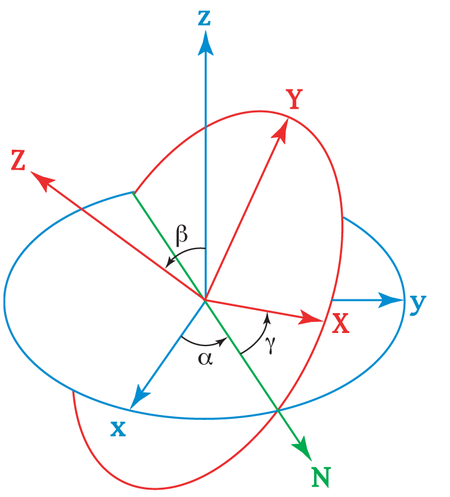
\includegraphics[width=0.9\linewidth]{img/eu_angles.png}
  \end{center}
    \caption{Углы Эйлера}
\end{wrapfigure}

Ортогональность матрицы $R$ даёт возможность описать её тремя независимыми параметрами. Один из вариантов сделать это -- углы Эйлера. 

Пусть начальная ПДСК $(x, y, z)$, а конечная -- $(X, Y, Z)$, при чём $xy \cap XY = ON$ -- линия узлов.
\begin{align*}
    1) \hspace{0.25cm}  \alpha &\colon Ox \to ON, &\text{ угол \textit{прецессии}}; \\
    2) \hspace{0.25cm}  \beta  &\colon Oz \to OZ, &\text{ угол \textit{нутации}}; \\
    3) \hspace{0.25cm}  \gamma &\colon OX \to ON, &\text{ угол \textit{собственного вращения}}.
\end{align*}
Повороты системы на эти углы называются прецессия, нутация и поворот на собственный угол (вращение). 

\phantom{42}

\noindent
Матричная запись углов Эйлера:
\begin{equation*}
    R_Z(\alpha) = \begin{pmatrix}
        \cos \alpha & - \sin \alpha & 0 \\
        \sin    a & \cos\alpha & 0 \\
        0 & 0 & 1\\
    \end{pmatrix},
\end{equation*}
\begin{equation*}
    R_X(\beta) = \begin{pmatrix}
        1 & 0 & 0 \\
        0 & \cos \beta & -\sin \beta \\
        0 & \sin \beta & \cos \beta \\
    \end{pmatrix},
    \hspace{1cm} 
    R_Z (\gamma) = \begin{pmatrix}
        \cos(\gamma) & - \sin \psi & 0 \\
        \sin \gamma & \cos \gamma & 0\\
        0 & 0 & 1
    \end{pmatrix}.
\end{equation*}

\begin{to_thr}[Теорема Эйлера]
     Произвольное перемещение твердого тела, имеющего неподвижную точку, можно осуществить посредством вращения вокруг некоторой оси, проходящей через эту точку. 
\end{to_thr}

\begin{to_thr}[Теорема Шаля]
     Самое общее перемещение твердого тела разлагается на поступательное перемещение, при котором произвольно выбранный полюс переходит из своего первоначального положения в конечное, и на вращение вокруг некоторой оси, проходящей через этот полюс. Это разложение можно совершить не единственным способом, выбирая за полюс различные точки тела; при этом направление и длина поступательного перемещения будут изменяться при выборе различных 
полюсов, а направление оси вращения и угол поворота вокруг нее не зависят от выбора полюса. 
\end{to_thr}

\begin{to_thr}[Теорема Моцци]
\label{thr_moz}
     Самое общее перемещение твердого тела является винтовым перемещением.
\end{to_thr}

\begin{to_con}[Теорема Бернулли-Шаля]
     Самое общее перемещение плоской фигуры в своей плоскости есть либо поступательное перемещение, либо вращение вокруг точки. Эта точка называется центром конечного вращения.
\end{to_con}Проведём два вектора $\vc{r}_A, \vc{r}_O$:
\begin{equation*}
    \vc{r}_A = \vc{r}_O + \vc{r} = \vc{r}_O + R(t) \vc{\rho}
    \hspace{0.5cm} \overset{d / dt}{\Rightarrow} \hspace{0.5cm} 
    \vc{v}_A = \vc{v}_O + \dot{R} \rho = \vc{v}_O + \dot{R} R^{-1}\vc{r}
\end{equation*}
но,
\begin{equation*}
    RR\T = E, \dot{R} R\T + R \dot{R}\T = 0, \dot{R} R\T = - R \dot{R}\T,
    (\dot{R} R^{-1})\T = - \dot{R} R^{-1}.
\end{equation*}

То есть $\dot{R} R^{-1}$ кососимметрична. Тогда пусть
\begin{equation*}
    \dot{R} R^{-1} = \Omega = \begin{pmatrix}
        0 & -\omega_z & w_y \\
        w_z & 0 & -\omega_x \\
        -\omega_y & \omega_x & 0\\
    \end{pmatrix}
\end{equation*}
Таким образом мы доказали следующую теорему.

\begin{to_thr}[формула Эйлера]
\label{eq_euler}
    Существует единственный вектор\footnote{
        Псевдоветор же, нет?
    } $\vc{\omega}$, называемый \textbf{угловой скоростью тела}, с помощью которого скорость $\vc{v}$ точки тела может быть представлена в виде
    \begin{equation*}
        \vc{v}_A = \vc{v}_O + \vc{\omega} \times \vc{r}
        \hspace{0.5cm} \text{--} \hspace{0.5cm} \text{\textbf{формула Эйлера}.}
    \end{equation*}
\end{to_thr}


Тогда, например, при постоянном радиус векторе верно, что
\begin{equation*}
    \vc{v}_A = \frac{d \vc{a}}{dt} = \vc{\omega} \times \vc{a},
    \hspace{0.5cm} \text{при условии $a = \const$}.
\end{equation*}

Можно вывести ускорение точки твёрдого тела
\begin{align*}
    \vc{\mathrm{w}}_A &= \vc{\mathrm{w}}_O + \frac{d \vc{\omega}}{dt} \times \vc{r} + \vc{\omega} \times \frac{d \vc{r}}{dt}, \\
    \vc{\mathrm{w}}_A &= \vc{\mathrm{w}}_O + \vc{\varepsilon} \times \vc{r} + \vc{\omega} \times \left(\vc{\omega} \times \vc{r} \right)
    \hspace{0.5cm} \text{--} \hspace{0.5cm} \text{\textbf{формула Ривальса},}
\end{align*}
где $\vc{\varepsilon} = d \vc{\omega} / d t$ -- \textit{угловое ускорение}. \subsubsection*{Тензор напряжений}
 В недеформированном теле молекулы находятся друг с другом в механическом и тепловом равновесии. При деформировании же взаимное расположение меняется и равновесие нарушается.
 \begin{to_def}
 	В результате возникают \textit{внутренние напряжения} --- силы, стремящиеся вернуть тело в равновесие, которые обуславливаются молекулярными силами, обладающими незначительным радиусом действия.
 \end{to_def}

Выделим в теле объём и рассмотрим суммарную действующую на него силу.
\textit{С одной стороны}, эта сила может быть представлена: $\int \vc{F} d V$, для $\vc{F}$ --- силы на единицу объема.
\textit{С другой стороны}, силы, с которыми действуют различные части объёма друг на друга не приведут к появлению никакой внешней силы.
Поэтому искомая полная сила будет состоят из сил действующих на объём со стороны окружающих его частей тела. В силу пренебрежимой малости радиуса молекулярных сил, внешние силы будут представленны как суммы сил на каждый элемент поверхности объёма.
\begin{to_def}
	$\int F_i d V = \int \frac{\partial \sigma^{i k}}{\partial x^k} = \oint \sigma^{i k} d f_k$. В последнем равенстве $\sigma^{i k}$ --- \textit{тензор напряжений}(симметричный). То есть $\sigma^{i k} d f_k$ есть $i$-ая компонента силы, действующей на элемент поверхности $d \vc{f}$.
\end{to_def}
Так, на единичную площадку, перпендикулярную оси $x$, действуют нормальная к ней сила $\sigma_{x x}$ и тангенциальные $\sigma_{y x}$ и $\sigma_{z x}$.
Знак силы $\sigma^{i k} d f_k$, которая является действующей на ограниченный поверхностью объём со стороны окружающих тел --- положительный. Для напряжений же извне, перед интегралом нужно поставить знак минус.

\subsubsection*{Всесторонее и не только сжатие}
При таком сжатии на каждую единицу поверхности тела действует одинаковое по величине давление $p$, направленное везде по нормали к поверхности внутрь объёма тела. 
А на элемент $d f_i$ действует сила $-p d f_i = \sigma^{i k} d f_k$. 
Таким образом при всестороннем сжатии тензор напряжений: $\sigma^{i k} = -p \delta^{i k}$.

В общем случае ещё и диагональные элементы тензора напряжений не нуль.
То есть, помимо нормальной силы, действуют ещё и тангенциальные <<скалывающие>> напряжения, стремящиеся сдвинуть параллельные элементы поверхности друг относительно друга.

В равновесии силы внутренних напряжений должны уравновешивать друг друга, то есть:
\begin{equation*}
	F_i = 0
	\hspace*{1 cm}
	\Rightarrow
	\hspace*{1 cm}
	\frac{\partial \sigma^{i k}}{\partial x^k} = 0.
\end{equation*}
И если тело находится в поле тяжести, то в равновесии:
\begin{equation*}
	\vc{F} + \rho g = 0
	\hspace*{1 cm}
	\Rightarrow
	\hspace*{1 cm}
	\frac{\partial\sigma^{ i k}}{\partial x^k} + \rho g^i - 0.
\end{equation*}

\subsubsection*{Внешние силы}
Обычно именно внешние силы вызывают деформацию, однако они будут просто входить в граничные условия к уравнениям равновесия. 
Внешняя сила $\vc{P}$ должна компенсироваться силой $\sigma^{i k} d f_k$:
\begin{equation*}
	P^i d f = - \sigma^{i k} d f_k = 0
	\hspace*{0.4 cm}
	\Rightarrow
	\hspace*{0.4 cm}
	d f_k = n_k d f
	\hspace*{0.4 cm}
	\Rightarrow
	\hspace*{0.4 cm}
	\sigma^{i k} n_k = P^i,
\end{equation*}
где $n$ --- единичный вектор нормали к площадке. Таким образом получили условие, которое должно выполняться на всей поверхности находящегося в равновесии тела.Пусть каждой точке среды соответсвует $\xi^1, \xi^2, \xi^3$, собственно $(\xi, t)$ -- \textit{лгранжевы переменные}. \textit{Закон движения среды} в таком случае это
\begin{equation}
    \vc{r} (\xi, t),
\end{equation}
скорость же
$$
    \vc{v} = \frac{\partial \vc{r}(\xi, t)}{\partial t},
    \hspace{0.5cm} 
    \vc{\mathrm{w}} = \frac{\partial \vc{v} (\xi, t)}{\partial t},
$$
и так далее.

Альтернативно можеем задать $(x, t)$ -- эйлерово описание. Тогда
$$
    \vc{v}(x, t), \vc{\mathrm{w}}(x, t) 
    \hspace{0.5cm} \text{-- поля скоростей и ускорений.}
$$

В частности, представляя движение по шоссе, полоса 1,2,3 и участок трассы -- эйлерово описание среды.
Если же мы будем следить за каждой машиной, то это будет лагранжево описание.\subsubsection*{Подход к деформации}
Под влиянием приложенных внешних сил твердые тела в той или иной степени \textit{деформируются}, то есть меняют свою форму и объём.
Рассмотрим точку деформируемого тела $\vc{r}(x^1,x^2,x^3)$, которая после деформации станет $\vc{r}'$.
\begin{to_def}
	$\vc{u} = \vc{r}' - \vc{r}$ --- \textit{вектор деформации}. Координаты $y^i$ смещенной точки могут быть выражены через $x^i$, таким образом $\vc{u}(x^i)$ полностью определяет деформацию тела.
\end{to_def}

Рассмотрим две близкие точки, расстояние между ними до деформации
$d (l')^2 = (d x^1)^2 + (d x^2)^2 + (d x^3)^2$, а 
после $d `l^2 = (d y^1)^2 + (d y^2)^2 + (d y^3)^2$.
Записав через деформацию (здесь $u_i = g_{i k}u^k$):
\begin{equation*}
	d (l')^2 = (d x^i + d u_i)^2
	\hspace*{0.4 cm}
	\Rightarrow
	\hspace*{0.4 cm}
	\left(d u_i = \frac{\partial u_i}{\partial x^k} d x^k \right)
	\hspace*{0.4 cm}
	\Rightarrow
	\hspace*{0.4 cm}
	d (l')^2 = d l^2 + 2 \frac{\partial u_i}{\partial x^k} d x^i d x^k + \frac{\partial u_i}{\partial x^k} \frac{\partial u_i}{\partial x^l} d x^k d x^l.
\end{equation*}
Поменяем во втором члене индексы $i$ и $k$, а в третьем $i$ и $l$:
\begin{equation*}
	d (l')^2 = d l^2 + 2 u_{i k} d x^i d x^k,
	\hspace*{1 cm}
	\text{где }
	u_{i k} = \frac{1}{2} \left(\frac{u_i}{\partial x^k} + \frac{u_k}{\partial x^i} + \frac{u_i}{\partial x^l} \frac{u_l}{\partial x^k}\right).
\end{equation*}
Как и всякий симметричный тензор, можно привести тензор $u_{i k}$ в каждой данной точке к главным осям. 
Это значит, что в каждой данной точке можно выбрать такую систему координат --- главные оси тензора, --- в которой из всех компонент 
$u_{i k}$ отличны от нуля только диагональные компоненты $u_{1 1}, u_{2 2}, u_{3 3}$.

При малых же деформациях, за исключением редких случаем, и вектор деформации оказывается малым, тогда можем пренебречь последним членом в полученном нами значении для тензора деформации:
\begin{to_def}[Тензор деформации в малом приближении]
	\begin{equation*}
		u_{i k} = \frac{1}{2} \left( \frac{\partial u_i}{\partial x^k} + \frac{\partial u_k}{\partial x^i}\right) .
	\end{equation*}
\end{to_def}

\subsubsection*{Изменение объёма при деформации}
Относительные удлинения элементов длины вдоль направлений главных осей тензора деформации с нашей точностью: $\sqrt{1 + 2 u_{i i}} - 1 \approx u_{ii}$.

Малый элемент объёма тогда претерпит следующее изменение:
\begin{equation*}
	d V' = d V(1 + u_{1 1})(1 + u_{2 2})(1 + u_{3 3}) d V (1 + u_{1 1} + u_{2 2} + u_{3 3})
	\hspace*{0.5 cm}
	\Rightarrow
	\hspace*{0.5 cm}
	u_{i i} = \frac{d V' - d V}{d V}.
\end{equation*}
Для несжимаемого тела, тогда $u_{i i}$ --- сумма диагональных компонент тензора в главных осях --- нулевая. Такая деформация называется \textit{сдвигом}.

\subsubsection*{Тензор скорости деформации}
\begin{to_def}
	\textit{Тензором скорости деформации}  назовём просто $\dot{u}_{i j} = \frac{d u_{i j} }{ d t} = \frac{1}{2}\left(\frac{\partial v_i}{\partial x^j} + \frac{\partial v_j}{\partial x ^i}\right)$.
\end{to_def}
Тогда рассмотрим движение элемента объёма тела во времени: $\vc{v} = \vc{v}(\vc{r} + \delta \vc{r})$, до первого члена малости:
\begin{equation*}
	\vc{v} = \vc{v}_0 + \frac{\partial \vc{v}}{\partial x^j} \delta x^j
	\hspace*{0.3 cm}
	\Rightarrow
	\hspace*{0.3 cm}
	\left(\vc{v}_0 = 0\right)
	\hspace*{0.3 cm}
	\Rightarrow
	\hspace*{0.3 cm}
	v_i = \frac{\partial v_i}{\partial x^j} \delta x^j = \frac{1}{2} \left(\frac{\partial v_i}{\partial x^j} + \frac{\partial v_j}{\partial x^i} \right) \delta x^j + \frac{1}{2} \left(\frac{\partial v_i}{\partial x^j} - \frac{\partial v_j}{\partial x^i} \right) \delta x^j.
\end{equation*}
Получаем уравнение, где с помощью замены, и вернув начальную скорость, явно можем показать, что
\begin{to_thr}[Теорема Гельмгольца]
	Тензор скоростей деформации можно разложить на сумму симметричного и кососимметричного:
	\begin{equation*}
	 	\vc{v} = \vc{v}_0 + u_{i j} \delta x^j e^i + \vc{\omega} \times \delta \vc{r}.
	 \end{equation*} 	
\end{to_thr} 

\subsubsection*{Обобщенный закон Гука}

Пусть $E$ -- модуль Юнга, $\mu$ -- коэффициент Пуассона. Тогда
$$
    u_{11} = \frac{\sigma_{11}}{E}, \hspace{0.5cm} 
    u_{22} = u_{33} = - \frac{\mu}{E} \sigma_{11}.
$$
Перепишем это в виду
$$
    u_{11} = \frac{\sigma_{11}}{E}  - \frac{\mu}{E} \sigma_{22} -
    \frac{\mu}{E} \sigma_{33} = \frac{1+\mu}{E} \sigma_{11} - \frac{\mu}{E} \tr \sigma.
$$
Или, в матричном виде
$$
    \begin{pmatrix}
        u_{11} & 0 & 0\\
        0 & u_{22} & 0 \\
        0 & 0 & u_{33}
    \end{pmatrix} =
    \frac{1+\mu}{E} 
    \begin{pmatrix}
        \sigma_{11} & 0 & 0\\
        0 & \sigma_{22} & 0 \\
        0 & 0 & \sigma_{33}
    \end{pmatrix} -
    \frac{\mu}{E} \tr \sigma 
    \begin{pmatrix}
        1 & 0 & 0\\
        0 & 1 & 0 \\
        0 & 0 & 1
    \end{pmatrix}.
$$
В тензорном виде
$$
    u_{ik} = \frac{1+\mu}{E} \sigma_{ik} - \frac{\mu}{E} \delta_{ik} \tr \sigma .
$$
Выразим $u$:
$$
    \tr u = \frac{1+\mu}{E} \tr \sigma - \frac{3\mu}{E} \tr \sigma
    \hspace{0.5cm} \Rightarrow \hspace{0.5cm} 
    \tr \sigma = \frac{E}{1-2\mu} \tr u.
$$
Так и получаем \textit{обобщенный закон гука}:
\begin{equation*}
    \sigma_{ik} = \frac{E}{1+\mu} \left[
        u_{ik} + \frac{\mu}{1 - 2\mu} \delta_{ik} \tr u 
    \right]
\end{equation*}\subsubsection*{Уравнение непрерывности}
\begin{to_def}[Предмет рассмотрения]
	Ввиду макроскопического рассмотрения \textit{жидкости}(газы) в гидродинамике представлется как сплошная среда, то есть малый элемент объёма жидкости содержит ещё достаточно больше количество молекул, относительно межмолекулярного расстояния.
\end{to_def}

Для описания движения жидкости требуется задать распределение скорости жидкости $\vc{v} = \vc{v}(x,y,z,t)$ и какие-либо её две термодинамические величины, как, например, плотность и давление. Важно отметить, что все эти величины относятся не к отдельной частице, а к точке в пространстве в определенное время.

\begin{to_thr}[Уравнение непрерывности]
\phantom{239}

\begin{proof}[$\triangle$]
	В маленьком объёме $V_{0}$ количество жидкости есть $\int_{V_0} \rho d V$.
	Через элемент поверхности, ограничивающей $V_0$, в единицу времени протекает $\rho \vc{v} \cdot d \vc{f}$ жидкости --- положительно или отрицательное число, в зависимости от того, вытекает или втекает жидкость соответственно.
	Тогда приравниваем для вытекания жидкости два наших рассуждения:
	\begin{equation*}
		- \frac{\partial}{\partial t} \int \rho d V =  \oint \rho \vc{v} \cdot d \vc{f}
		\hspace*{0.5 cm} 
		\Rightarrow 
		\hspace*{0.5 cm}
		\int \left(\frac{\partial \rho}{\partial t} + \div \rho \vc{v}\right)d V = 0
		\hspace*{0.5 cm}
		\Rightarrow
		\hspace*{0.5 cm}
		\frac{\partial \rho}{\partial t} + \div \rho \vc{v} = 0.
	\end{equation*}
	Последнее следует из того, что равенство должно иметь для любого объёма, таким образом получили искомое \textit{уравнение непрерывности}.
\end{proof}
	
\end{to_thr}

\subsubsection*{Уравнение Эйлера}

\begin{to_thr}[Уравнение Эйлера]
\phantom{239}

\begin{proof}[$\triangle$]
	Выделим в жидкости некоторый объём, полная сила, действующая на этот объём: $- \oint p d \vc{f} = - \int \grad p d V$, где интеграл из взятого по поверхности объёма преобразуется в сам рассматриваемый объём.
	Таким образом получили, что на единицу объёма жидкости будет действовать сила:
	\begin{equation*}
		\rho \frac{d \vc{v}}{d t} = - \grad p.
	\end{equation*}
	Однако стоящая здесь скорость определяет изменение скорости именно элемента объёма, а не точки в пространстве.
	Запишем это изменение скорости:
	\begin{equation*}
		d \vc{v} 
		=
		 \frac{\partial \vc{v}}{\partial t} d t + \frac{\partial \vc{v}}{\partial x^i} d x^i 
		= 
		\frac{\partial \vc{v}}{\partial t} d t + (d \vc{r} \cdot \nabla) \vc{v}
		\hspace*{1 cm}
		\Rightarrow
		\hspace*{1 cm}
		\frac{\partial \vc{v}}{\partial t} + (\vc{v} \nabla) \vc{v} = - \frac{1}{\rho} \grad p.
	\end{equation*}
	Последнее и есть искомое уравнение Эйлера.
\end{proof}
\end{to_thr}

Если же жидкость движется во внешнем поле тяжести, то, на каждый элемент объёма будет действовать сила, которая просто добавится к изначальному уравнению: 
\begin{equation*}
	\frac{\partial \vc{v}}{\partial t} + (\vc{v} \nabla) \vc{v} = - \frac{\nabla p}{\rho} + \vc{g}.
\end{equation*}

\subsubsection*{Уравнение Навье-Стокса}

Чтобы нормально учесть вязкость, нужно поговорить про \textit{поток импульса}.
Импульс единицы объёма жидкости есть $\rho \vc{v}$, скорость изменения его компоненты:
\begin{equation*}
	\frac{\partial}{\partial t} \rho v^i = \rho \frac{\partial v^i}{\partial t} + \frac{\partial \rho}{\partial t} v^i.
\end{equation*}
Уравнения непрерывности и Эйлера запишутся в тензорном виде:
\begin{equation*}
	\frac{\partial \rho}{\partial t} = - \frac{\partial (\rho v^k)}{\partial x^k},
	\hspace*{0.5 cm}
	\hspace*{0.5 cm}
	\frac{\partial v^i}{\partial t} = - v^k \frac{\partial v^i}{\partial x^k} - \frac{1}{\rho} \delta^{i k} \frac{\partial p}{\partial x^k}.
\end{equation*}
Тогда получим:
\begin{equation*}
	\frac{\partial}{\partial t} \rho v^i 
	= 
	- \rho v^k \frac{\partial v^i}{\partial x^k} -  \delta^{i k} \frac{\partial p}{\partial x^k} - v^i \frac{\partial \rho v^k}{\partial x^k} 
	=
	-\delta^{i k} \frac{\partial p}{\partial x^k} - \frac{\partial}{\partial x^k} \rho v^i v^k
	= - \frac{\partial \Pi^{i k}}{\partial x^k}.
\end{equation*}
\begin{to_def}
	$\Pi^{i k} $ --- \textit{тензор плотности потока импульса}:
	$
		\Pi^{i k} = p \delta^{i k} + \rho v^i v^k.
	$
\end{to_def}

Таким образом уравнение Эйлера у нас записалось в виде:
$
	\frac{\partial}{\partial t} \rho v^i = - \frac{\partial \Pi^{i k}}{\partial x^k}.
$
Поток импульса представляет собой чисто обратимый перенос импульса, связанный с просто механическим передвижением различных участков жидкости и с действующими в жидкости силами давления.
\textit{Вязкость} (внутреннее трение) жидкости проявляется в наличии ещё дополнительного, необратимого переноса импульса из мест с большой скоростью в места с меньшей.

Поэтому уравнение движения вязкой жидкости можно получить, прибавив к идеальному потоку импульса дополнительный член $\sigma^{i k}_{visc}$, определяющий такой вязкий перенос:
$
\Pi^{i k} = p \delta^{i k} + \rho v^i v^k - \sigma^{i k}_{visc} = - \sigma^{i k} + \rho v^i v^k.
$
\begin{to_def}
	Таким образом: $\sigma^{i k} = - p \delta^{i k} + \sigma^{i k}_{visc}$ называют \textit{тензором напряжений}, а $\sigma^{i k}_{visc}$ --- вязким тензором напряжений.
\end{to_def}

Чтобы написать выражение для вязкого напряжения сделаем пару оговорок. 
\textit{Во первых}, градиенты скорости движения участков жидкости относительно друг друга не велики, тогда $\sigma^{i k}_{visc}$ зависит лишь от первых производных скорости по координатам, линейно. \textit{Во вторых}, не зависящие от первых производных величины должны обращаться в нуль как для скорости потока $\vc{v} = \const$ и тензор должен быть нулевым. \textit{В третьих}, $\sigma^{i k}_{visc} = 0$ когда жидкость совершает целое равномерное вращение, поскольку никакого внутреннего трения тогда не будет.
Для такого равномерного вращения с $\vc{v} = [\vc{\omega} \vc{r}]$ линейными комбинациями производных обращающимися в нуль будут: $\frac{\partial v^i}{\partial x^k} + \frac{\partial v^k}{\partial x^i}$.

Это всё даёт нам мотивацию для не шибко сильных потоков несжимаемой жидкости согласится с Сэром Исааком Ньютоном, и написать тензор вязкого напряжения, как \textit{тензор скорости деформации}:
\begin{equation*}
	\sigma^{i k}_{visc} = \eta \left(\frac{\partial v^i}{\partial x^k} + \frac{\partial v^k}{\partial x^i}\right),
	\hspace*{1 cm}
	\Rightarrow
	\hspace*{1 cm}
	\sigma^{i k} = - p \delta^{i k} + \eta \left(\frac{\partial v^i}{\partial x^k} + \frac{\partial v^k}{\partial x^i}\right).
\end{equation*}
А уравнение Эйлера тогда для несжимаемой жидкости запишется:
\begin{equation*}
	\rho \left(\frac{\partial v^i}{\partial t} + v^k \frac{\partial v^i}{\partial x^k}\right)
	=
	- \delta^{i k} \frac{\partial p}{\partial x^k} + \frac{\partial}{\partial x^k} \left[\eta \left(\frac{\partial v^i}{\partial x^k} + \frac{\partial v^k}{\partial x^i}\right)\right].
\end{equation*}
а в более человеческом, привычном глазу, виде:
\begin{equation*}
	\frac{\partial \vc{v}}{\partial t} + (\vc{v} \triangle) \vc{v} = - \frac{1}{\rho} \grad p + \frac{\eta}{\rho} \Delta \vc{v}.
\end{equation*}
\begin{to_def}
	Коэффициент $\eta$ называется --- \textit{динамическим коэффициентом вязкости}, а отношение $\eta/\rho = \nu$ --- \textit{кинематической вязкостью}.
\end{to_def}
\begin{to_def} 
    \textit{Обобщенная сила} $Q_k$ -- величина коэффициента $\partial q^k$ при вариации $\delta A$, то есть $\delta A = Q_k \delta q^k$.
\end{to_def}

\begin{to_thr}[Уравнения Лагранжа второго рода]
     Каждая механическая система характеризуется определенной функцией $L(q, \dot{q}, t)$. Для голономных системы с конфигурационном многообразием степени $n$, верно что
     \begin{equation*}
         \frac{d}{dt} \frac{\partial L}{\partial \dot{q}_k} - \frac{\partial L}{\partial q_k} = 0, \hspace{0.5cm} k = 1, \ldots, n.
     \end{equation*}
     Где для потенциальных систем $L = T - \Pi$. В более общем случае можно записать, что
     \begin{equation*}
         \left(\frac{d }{d t} \frac{\partial T}{\partial \dot{q}^k} - \frac{\partial T}{\partial q^k} - Q^k\right)\delta q^k = 0, \hspace{0.5cm} 
         Q^k = - \frac{\partial \Pi}{\partial q^k}.
     \end{equation*}
\end{to_thr}

\begin{proof}[$\triangle$]
Запишем второй закон Ньютона:
$
    \left(
        m_i \vc{\mathrm{w}}_i = \vc{F}_i + \vc{R}_i
    \right)\big|_{\cdot \d \vc{r}_i}
$
, где $\vc{R}_i$ -- реакции связи. Хотим записать уравнение в общековариантном виде.
То есть мы <<замораживаем>> время, так чтобы $\vc{R} \cdot \delta \vc{r} = 0$. На таких перемещениях работа реакция связи равна 0.
\begin{align*}
    \bigg[
        \sum m_i \left(\vc{\mathrm{w}}_i \cdot \frac{\partial \vc{r}_i}{\partial q^k} \right)
        -
        \left(\vc{F}_i \cdot \frac{\partial \vc{r}_i}{\partial q^k} \right)
        -
        \underbrace{
        \left(
            \vc{R}_i \cdot \frac{\partial \vc{r}_i}{\partial q^k} 
        \right)}_{\cdot \delta q^k \to 0}
    \bigg] \cdot \delta q^k &= 0;
    \\
    \left[
        \frac{d}{dt} \frac{\partial }{\partial \dot{q}^k} \sum  \frac{m_i v_i^2}{2} 
        -
        \frac{\partial }{\partial q^k} \sum \frac{m_i v_i^2}{2} -
        \sum \vc{F}_i \frac{\partial \vc{r}_i}{\partial q^k} 
    \right] \delta q^k &= 0
    , \hspace{0.5cm} \Rightarrow \hspace{0.5cm} 
    \sum_k
    \left[
        \frac{d}{dt} \frac{\partial T}{\partial \dot{q}^k} 
        - \frac{\partial T}{\partial q^k} - Q_k
    \right] \delta q^k = 0.
\end{align*}
Проблема остается в неголономных системах, где $\delta q^k$ не являются независимыми, получается, что уравнения Лагранжа справедливы для голономных систем.

Вспоминая, что
\begin{equation*}
    \delta  A = \sum_i \vc{F}_i \cdot \delta \vc{r}_i =
    \sum_i \left(\vc{F}_i \cdot \frac{\partial \vc{r}_i}{\partial q^k}\right) \delta q^k \overset{\text{\red{?}}}{=} 
    \sum_k 
    \frac{\delta A_k}{\delta q^k} \delta q^k = Q_k \delta q^k.
\end{equation*}
Тогда пусть $\Pi (q, t) \colon Q_k = - \partial \Pi / \partial q^k$.  Тогда
\begin{equation*}
    \frac{d}{dt} \frac{\partial (T-\Pi)}{\partial \dot{q}^k} - \frac{\partial (T - \Pi)}{\partial q^k}  = 0,
    \hspace{0.5cm} \Rightarrow \hspace{0.5cm} 
    \frac{d}{dt} \frac{\partial L}{\partial \dot{q}^k} - \frac{\partial L}{\partial q^k} = 0, \hspace{0.5cm} k = 1, \ldots, n.
\end{equation*}
То есть получили систему уравнений на $2n$ переменных.
\end{proof}



Подставим разложение кинетической энергии в уравнения Лагранжа, оставив только слагаемые с обобщёнными ускорениями $f_j (q, \dot{q}, t) = a_{jk} \ddot{q}^j$. 
\begin{equation*}
    T = \frac{1}{2} \sum_\nu m_\nu \dot{\vc{r}}_\nu^2 = \frac{1}{2} \sum_\nu
    \left(
        \frac{\partial \vc{r}_\nu}{\partial q^j} \dot{q}^j + \frac{\partial \vc{r}_\nu}{\partial t} 
    \right)^2 = 
    \frac{1}{2} 
    \bigg[
    \underbrace{
        a_{jk} \dot{q}^j \dot{q}^k
    }_{
        2T_2
    } +
    \underbrace{
        a_j \dot{q}^j
    }_{
        2T_1
    } +
    \underbrace{
        a_0
    }_{
        2T_0
    }
    \bigg],
\end{equation*}
где коэффициенты, соответственно, равны 
\begin{equation*}
    a_{jk}(q, t) = \sum_\nu m_\nu \frac{\partial \vc{r}_\nu}{\partial q^j} \cdot \frac{\partial \vc{r}_\nu}{\partial q^k},
    \hspace{0.5cm} 
    a_j(q, t) = \sum_\nu m_\nu \frac{\partial \vc{r}_\nu}{\partial q^j} \cdot \frac{\partial \vc{r}_\nu}{\partial t},
    \hspace{0.5cm} 
    a_0 = \sum_\nu m_\nu 
    \left(
    \frac{\partial \vc{r}_\nu}{\partial t} 
            \right)^2.
\end{equation*}
Для склерономных систем $\partial \vc{r}_\nu / \partial t = 0$, соотвественно $T = a_{jk} \dot{q}^j \dot{q}^k$, при чём $a_{jk} \equiv a_{jk} (q)$.

Теперь подставим значение $T$ в уравнения Лагранжа, и получим, что
$
    a_{ik} \ddot{q}^k = f_i,
$
где $f_1 = f_1(q, \dot{q}, t)$. Уравнений в системе $n$, причём $a_{jk}$ является положительно определенной формой\footnote{
    \red{Требует отдельного доказательства.}
}, соответственно невырожденной. 

\begin{to_thr} 
    Уравнения Лагранжа второго рода разрешимы относительно обобщенных ускорений 
\end{to_thr}
Пусть есть также непотенциальные силы, часть обобщенных сил, соответстующих непотенциальным силам, обозначим $Q_i^*$, тогда
\begin{equation*}
    Q_1 = - \frac{\partial \Pi}{\partial q^i} + Q_i^*,
    \hspace{0.5cm} \Rightarrow \hspace{0.5cm} 
    \frac{d }{d t} \frac{\partial T}{\partial \dot{q}^i} - 
    \frac{\partial T}{\partial q^i} 
    =
    - \frac{\partial \Pi}{\partial q^i} + Q_i^*.
\end{equation*}
Найдём производную по времени от кинетической энергии
\begin{equation*}
    \frac{d T}{d t} = 
    \frac{\partial T}{\partial \dot{q}^i} \ddot{q}^i + \frac{\partial T}{\partial q^i} \dot{q}_i + \frac{\partial T}{\partial t}  =
    \frac{d }{d t} \left(
        \frac{\partial T}{\partial \dot{q}^i} \dot{q}^i
    \right) - \left(
        \frac{d }{d t} \frac{\partial T}{\partial \dot{q}^i} - \frac{\partial T}{\partial q^i} 
    \right) \dot{q}^i + \frac{\partial T}{\partial t}.
\end{equation*}
По \textit{теореме Эйлера об однороных функциях} для $f(x_1, \ldots, x_n)$ $k$-й степени верно что
\begin{equation*}
    \frac{\partial f}{\partial x^i} x^i = kf,
    \hspace{0.5cm} \Rightarrow \hspace{0.5cm} 
    \frac{\partial T}{\partial \dot{q}^i} \dot{q}^i = 2 T_2 + T_1.
\end{equation*}
В таком случае последнее равеноство перепишется, как
\begin{align*}
    \frac{d T}{d t} 
    &=
    \frac{d }{d t} (2 T_2 + T_1) + \frac{\partial \Pi}{\partial q^i} \dot{q}^i - Q_i^* \dot{q}^i + \frac{\partial T}{\partial t} 
    = \\ &= 
    \frac{d }{d t} (2 T_2 + 2 T_1 + 2 T_0) - \frac{d }{d t} (T_1 + 2 T_0) + \frac{d \Pi}{d t} - \frac{\partial \Pi}{\partial t} - Q_i^* \dot{q}^i + \frac{\partial T}{\partial t}.
\end{align*}
Таким образом мы доказали следующую теорему.

\begin{to_thr}
     Полная мехническая энергия голономной системы $E = T+ \Pi$ изменяется следующим образом:
     \begin{equation*}
         \frac{d E}{d t} = N^* + \frac{d }{d t} (T_1 + 2 T_0) + \frac{\partial \Pi}{\partial t} - \frac{\partial T}{\partial t}.
     \end{equation*}
     Где $N^* = Q^*_i \dot{q}^i$ -- мощность непотенциальных сил.
\end{to_thr}


\begin{to_def} 
    Голономная склерономная система с  $\Pi \equiv \Pi(q)$ называется \textit{консервативной}, при чём $d E / d t = 0$.
\end{to_def}

\subsubsection*{Гироскопические силы}


\begin{to_def} 
    Непотенициальные силы называют \textit{гироскопическими}, если их мощность равна $0$. 
\end{to_def}


Пусть $Q^*_i = \gamma_{ik} \dot{q}^k$. Если $\gamma_{ik} = -\gamma_{ki}$, то силы $Q^*_i$ гиросокопические, соответсвенно кососимметричность $\gamma_{ik}$ необходима и достаточна.

Более того, имеет место равеноство

\vspace{-25pt}
\begin{equation*}
    \sum_\nu \vc{F}_\nu \cdot \vc{v}_\nu = \sum_\nu \vc{F}_\nu \cdot
    \left(
        \frac{\partial \vc{r}_\nu}{\partial q^i} \dot{q}^i + \frac{\partial \vc{r}_\nu}{\partial t} 
    \right) 
    =
     \bigg(
     \overbrace{
     \sum_\nu \vc{F}_\nu \cdot \frac{\partial \vc{r}_\nu}{\partial q^i}
     }^{
     Q_i
     }
      \bigg)
     \dot{q}^i + \sum_\nu \vc{F}_\nu \cdot \frac{\partial \vc{r}_\nu}{\partial t},
     \hspace{0.25cm} \overset{\partial \vv{r}_\nu / \partial t = 0}{=}  \hspace{0.25cm} 
     \sum_\nu \vc{F}_\nu \cdot \vc{v}_\nu = Q_i \dot{q}^i.
\end{equation*}
Поэтому для склерономных систем $N^* = 0$ выражается в $\sum_\nu \vc{F}_\nu^* \cdot \vc{v}_\nu = 0$.

\subsubsection*{Диссипативные силы}

\begin{to_def} 
    Непотенциальные силы называются диссипативными, если их $N^* \leq 0$, но $N^* \not \equiv 0$. При $\Pi = \Pi(q)$ и диссипативности сил $d E / dt \leq 0$, тогда система называется диссипативной. В случае определенно-отрицательной $N^* (\dot{q})$ дисспация называется \textit{полной}, а в случае знакопостоянной отрицательной $N^*$ \textit{частичной}.
\end{to_def}

\begin{to_def} 
    \textit{Диссипативной функцией Рэлея} называется  положительная квадратичная форма $R$ такая, что
    \begin{equation*}
        R = \frac{1}{2} b_{ik} \dot{q}^i \dot{q}^k,
        \hspace{1cm}
        Q^*_i = - \frac{\partial R}{\partial \dot{q}^i}  = - b_{ik} \dot{q}^k.
    \end{equation*}
    Тогда для склерономной системы можность $N^*$ непотенциальных сил равна
    \begin{equation*}
        \sum_\nu \vc{F}_\nu^* \cdot \vc{v}_\nu = Q_i^* \dot{q}^i = - 2 R \leq 0.
    \end{equation*}
\end{to_def}




Путь существует функция $V (q, \dot{q}, t)$ такая, что обобщенные силы $Q_i$ определяются по формулам
\begin{equation*}
    Q_i = \frac{d }{d t} \frac{\partial V}{\partial \dot{q}^i} - \frac{\partial V}{\partial q^i}.
\end{equation*}
Тогда функция $V$ называется обобщенным потенциалом. Действительно, при $L = T - V$ уравнения движения запишутся в той же форме. Дифференцируя по времени выясним, что
\begin{equation*}
    Q_i = \frac{\partial^2 V}{\partial \dot{q}^i \partial \dot{q}^k} \ddot{q}^k + f_i,
\end{equation*}
где $f_i \equiv f_i ( q,\dot{q}, t)$. Но так как зависимость $Q_i(\ddot{q})$ это странно, то
\begin{equation*}
    V =  A_i(q, t) \dot{q}^i + V_0(q, t).
\end{equation*}
Тогда обобщенные силы
\begin{equation*}
    Q_i = \frac{d A_i}{d t} - \frac{\partial }{\partial q^i} \left(
        A_k \dot{q}^k  + V_0
    \right) = - \frac{\partial V_0}{\partial q^i} + \frac{\partial A_i}{\partial t} +
    \left(
        \frac{\partial A_i}{\partial q^k} - \frac{\partial A_k}{\partial q^i} 
    \right) \dot{q}^k.
\end{equation*}
Если $\partial A_i / \partial t = 0$, то $Q_i$ складываются из потенциальных $\partial V_0 / \partial q_i$ и гироскопических $Q_i^* = \gamma_{ik} \dot{q}^k$, где $\gamma_{ik} = \partial_k A_i - \partial_i A_k$. Если система склерономна и $V_0 \neq V_0(t)$, то $T+V_0$ остается постоянной.

В случае существования обобщенного потенциала $L$ всё так же многочлен второй степени относительно $q, \ \dot{q}$, при чём $L_2 = T_2$, так что уравнения остаются разрешимы относительно обобщенных ускорений.


\subsubsection*{Натуральные системы}

\begin{to_def} 
    Системы, в которых силы имеют обычный $\Pi(q_i, t)$ или обобщенный $V(q^i, \dot{q}^i, t)$ потенциал, называются \textit{натуральными}. В таких системах $L = T - \Pi$.
    Более общие системы $L(q^i, \dot{q}^i, t)$ не представимы в виде однако при выполнении условия, 
    \begin{equation*}
         \det \left[
            \frac{\partial^2 L}{\partial \dot{q}^i \partial \dot{q}^k} 
         \right] \neq 0,
    \end{equation*}
    то есть ненулевого гессиана лагранжиана, 
    уравнения Лагранжа остаются разрешимы относительно обобщенных ускорений.
\end{to_def}


\subsubsection*{Первые интегралы \textnormal{(\red{воообще про первые интегралы читайте билет №35})}}

\begin{to_def} 
    \textit{Первым интегралом} системы дифференциальных уравнений называется функция $f(q,\ \dot{q}, \ t)$  (фазовых переменных), сохраняющая свои значения на любом решении этой системы.
\end{to_def}

\begin{to_def} 
    Распространенным первым интегралом являются \textit{цциклические} интегралы $\partial L / \partial \dot{q}^k$. Переменная $q^k$ называется \textit{циклической}, если она не входит в выражение для $L$.  
\end{to_def}






\subsubsection*{Преобразование Лежандра}

\begin{to_def} 
    В уравнениях Лагранжа второго рода движения голономной системы в потенциальном поле сил, функция Лагранжа зависит от $q, \ \dot{q}, \ t$ -- \textit{переменные Лагранжа}.
    Если в качестве параметров взять $q, \ p, \ t$, где $p_i$ -- \textit{обобщенные импульсы}\footnote{
        Обобщенный импульс $p_i$ -- ковектор, а  не вектор!
    }, определяемые как
    $
        p_i = {\partial L}/{\partial \dot{q}^i}.
    $
    То получим набор $q, \ p, \ t$ -- \textit{переменные Гамильтона}. 
\end{to_def}

В силу невырожденности $\partial L / (\partial \dot{q}^i \partial \dot{q}^j) = J_{p}$, то есть по \textit{теореме о неявной функции} эти равенства разрешимы относительно переменных $\dot{q}^i$. Через преобразование Лежандра естестественно ввести функцию
\begin{equation*}
    H(q, p, t) = p_i \dot{q}^i - L(q, \dot{q}, t),  \hspace{0.5cm} \dot{q} \equiv \dot{q}(q, p, t).
\end{equation*}

\subsubsection*{Уравнения Гамильтона}
% Маркеев, п.149.

Полный дифференциал функции Гамильтона можем выразиь двумя способами:
\begin{equation*}
    \left.\begin{aligned}
        d H &= \frac{\partial H}{\partial q^i} \d q^i + \frac{\partial H}{\partial p_i} \d p_i + \frac{\partial H}{\partial t} \d t,
        \\
        dH &= \dot{q}^i \d p_i - \frac{\partial L}{\partial q^i} \d q^i - \frac{\partial L}{\partial t} \d t.
    \end{aligned}\right\}
    \hspace{0.7cm} \Rightarrow \hspace{0.7cm} 
    \left.\begin{gathered}
        \frac{\partial H}{\partial t} = - \frac{\partial L}{\partial t} \\
        \frac{\partial H}{\partial p_i} = \dot{q}^i, \ \ 
        \frac{\partial H}{\partial q^i} = - \frac{\partial L}{\partial q^i}
    \end{gathered}\right.
    \hspace{0.7cm} \Rightarrow \hspace{0.7cm} 
    \left\{\begin{aligned}
        \frac{d q^i}{d t} &= \frac{\partial H}{\partial p_i}, \\
        \frac{d p_i}{d t} &= - \frac{\partial H}{\partial q^i}.    
    \end{aligned}\right.
\end{equation*}
Эти уравнения называются \textit{уравнениями Гамильтона}, или \textit{каноническими уравнениями}.


\subsubsection*{Физический смысл функции Гамильтона}

Пусть система натуральна, тогда $L = L_2 + L_1 + L_0$, и, соответсвенно,
\begin{equation*}
    H = \frac{\partial L}{\partial \dot{q}^i} \dot{q}^i - L.
\end{equation*}
По теореме Эйлера об однородных функциях
\begin{equation*}
    \frac{\partial L_2}{\partial \dot{q}^i} \dot{q}^i = 2 L_2,
    \hspace{1cm} 
    \frac{\partial L_1}{\partial \dot{q}^i} \dot{q}^i = L_1,
    \hspace{0.5cm} \Rightarrow \hspace{0.5cm} 
    H = L_2 - L_0.
\end{equation*}
пусть $T = T_2 + T_1 + T_0$, если силы имеют обычный потенциал $\Pi$, то $L_0 = T_0 - \Pi$, 
\begin{equation*}
    H = T_2 - T_0 + \Pi.
\end{equation*}
Если же силы имеют обобщенный потенциал $V = V_1 + V_0$, то $L_0 = T_0 - V_0$, и
\begin{equation*}
    H = T_2 - T_0 + V_0.
\end{equation*}
В случае натуральных и склерономных систем $T_1 = T_0 = 0$ и $T = T_2$, тогда $H = T + \Pi$. Т.е. для натуральных склерономных систем с обычным потенциалом сил функция Гамильтона $H$ представляет собой полную механическую энергию.

\subsubsection*{Интеграл Якоби}

Найдём полную производную $H$ по времени,
\begin{equation*}
    \frac{d H}{d t} = \frac{\partial H}{\partial q^i} \dot{q}^i + \frac{\partial H}{\partial p_i} \dot{p}_i + \frac{\partial h}{\partial t} = 
    \frac{\partial H}{\partial q^i} \frac{\partial H}{\partial p_i} - \frac{\partial H}{\partial p_i} \frac{\partial H}{\partial q^i} + \frac{\partial H}{\partial t} = \frac{\partial H}{\partial t},
    \hspace{0.5cm} \Rightarrow \hspace{0.5cm} 
    \frac{d H}{d t} = \frac{\partial h}{\partial t}.
\end{equation*}
Система называется \textit{обобщенно консервативной}, если $\partial H / \partial t = 0$, т.е $H(q^i, p_i) = h$, собственно, $H$ называют \textit{обобщенной полной энергией}, а поледнее равенство -- \textit{обобщенным интегралом энергии}.


\begin{to_def} 
    Для натуральной системы с обычным потенциалом сил, если $\partial H/ \partial t =0$, то
    \begin{equation*}
         H = T_2 - T_0 + \Pi = h = \const.
     \end{equation*} 
     Соотноешние, где $h$ -- произвольная постоянная, называют \textit{интегралом Якоби}.
\end{to_def}

Есть и другая формулировка для интеграла Якоби голономной склерономной системы. Действительно, при $\partial L / \partial t = 0$, интеграл Якоби перейдёт в
\begin{equation*}
    \frac{\partial H}{\partial t} = 0,
    \hspace{0.25cm} \Rightarrow \hspace{0.25cm} 
    \frac{d }{d t} \left(
        \frac{\partial L}{\partial \dot{q}^i} \dot{q}^i
    \right) = 0,
    \hspace{0.25cm} \Rightarrow \hspace{0.25cm} 
    \frac{\partial L}{\partial \dot{q}^i} \dot{q}^i = \const.
\end{equation*}



\subsubsection*{Уравнения Уиттекера}


Если $\partial H / \partial t = 0$, то $H(q, p) = h$, где $h = \const$ определяемая из н.у. В $2n$-мерном пространстве $q, \ p$ интеграл Якобми задаёт гиперповерхность, рассмотрим движение с $H = h$.

Такое движение описывается системой с $2n-2$ уравнений, причём она может быть записана в виде канонических уравнений. Пусть $\partial H / \partial p_1 \neq 0$, тогда
\begin{equation*}
    p_1 = - K(q^1, \ldots, q^n, p_2, \ldots, p_n, h),
    \hspace{0.5cm} \Rightarrow \hspace{0.5cm} 
    \left\{\begin{aligned}
        \dot{q}^i = \frac{\partial H}{\partial p_i}, \\
        \dot{p}_j = - \frac{\partial H}{\partial q^j}        
    \end{aligned}\right.
    \hspace{0.5cm} \Rightarrow \hspace{0.5cm} 
    \frac{d q^j}{d q^1} = \frac{
    \left(\dfrac{\partial H}{\partial p_j} \right)
    }{
    \left(\dfrac{\partial H}{\partial p_1} \right)
    },
    \hspace{0.5cm} 
    \frac{d p_j}{d q^1} = - \frac{
    \left(\dfrac{\partial H}{\partial q^j}\right)
    }{
    \left(\dfrac{\partial H}{\partial p_1} \right)
    },
\end{equation*}
для $j = 2,\ 3,\ \ldots,\ n$. Подставляя $p_1$ получим
\begin{align*}
    &\frac{\partial H}{\partial q^j} - \frac{\partial H}{\partial p_1} \frac{\partial K}{\partial q^j} = 0,
    &(j = 2, \ 3, \ \ldots, n);
    \\
    &\frac{\partial H}{\partial p_j} - \frac{\partial H}{\partial p_1} \frac{\partial K}{\partial p_j}  = 0,
    &(j = 2, \ 3, \ \ldots, n).
\end{align*}
Допиливая до надлежащего вида, окончательно находим
\begin{equation*}
    \frac{d q^j}{d q^1} = \frac{\partial K}{\partial p_j},
    \hspace{1cm} 
    \frac{d p_j}{d q^1} = - \frac{\partial K}{\partial q^j},
    \hspace{1cm} 
    (j = 2, \ 3, \ \ldots, n).
\end{equation*}
Эти уравнения описывают движения системы при $H = h = \const$, и называются \textit{уравнениями Уиттекера}. 

\subsubsection*{Уравнения Якоби}


Уравнения Уиттекера имеют структуру уравнений Гамильтона, соответственно их можно зписать в виде уравнений типа Лагранжа, при гессиане $K$ по $p$ неравным 0. Пусть $P$ -- преобразование Лежандра функции $K$ по $p_j$ ($j = 2, \ 3,\ \ldots,\ n$). Тогда
\begin{equation*}
    P = P(q^2, \ldots, q^n, \tilde q^2, \ldots, \tilde q^n, q^1, h) = \sum_{j = 2}^{n} \tilde q^j p_j - K,
\end{equation*}
где $\tilde q^{j} = d q^j / d q^1$. Величины $p_j$ выражаются через $\tilde q^2, \ \ldots, \ \tilde q_n$ из уравнений 
\begin{equation*}
    \tilde q^j = \frac{\partial K}{\partial p_j}, \hspace{0.5cm} 
    (j = 2, \ 3, \ \ldots, n),
\end{equation*}
т.е. из первых $n-1$ уравнений Уиттекера. При помощи функции $P$ эти уравнения могут быть записаны в эквивалентной форме:
\begin{equation*}
    \frac{d }{d q^1} \frac{\partial P}{\partial q_j'} - \frac{\partial P}{\partial q^j} = 0
    \hspace{1cm} (j = 2,\ 3,\ \ldots,\ n).
\end{equation*}
Это уравнения типа Лагранжа, называются \textit{уравнениями Якоби}.

Преобразовывая выражение для $P$ найдём, что
\begin{equation*}
    P = \sum_{j=2}^{n} q_j \tilde q^j + p_1 = 
    \sum_{i=1}^{n} p_1 \tilde q_i = \frac{1}{\dot{q}^1} \sum_{i=1}^{n} p_i \dot{q}^i = \frac{1}{\dot{q}^1} (L+H).
\end{equation*}
Тогда в случае консервативной системы $L = T - \Pi$, $H = T + \Pi$, и
\begin{equation*}
    P = \frac{2T}{\dot{q}^1},
    \hspace{0.5cm} 
    T = \frac{1}{2} a_{ik} \dot{q}^i \dot{q}^k = (\dot{q}^1)^2 G(q^1, \ldots, q^n, \tilde q^2, \ldots, \tilde q^n),
    \hspace{0.5cm} 
    G = \frac{1}{2} a_{ik} \tilde q^i \tilde q^k.
    \hspace{0.5cm} \Rightarrow \hspace{0.5cm} 
    \tilde q^1 = \sqrt{\frac{h-\Pi}{G} }
\end{equation*}
Таким образом выражение для 
\begin{equation*}
    P = 2 \sqrt{(h-\Pi)G }.
\end{equation*}


\subsubsection*{Скобки Пуассона}

\begin{to_def} 
    Пусть $u$, $v$ $\in C^2(q, p, t)$, тогда выражение
    \begin{equation*}
        \{u, v\}  
        =
        \frac{\partial u}{\partial q^i} \frac{\partial v}{\partial p_i} -
        \frac{\partial u}{\partial p_i} \frac{\partial v}{\partial q^i}
    \end{equation*}  
    называют \textit{скобкой Пуассона} функций $u$ и $v$.
\end{to_def}

Вообще, можно было бы ввести алгебры Ли и показать, что пространство гладких функций $f(t, x, p)$ является алгеброй Ли относительно скобки Пуассона. Выражается это в выполнение следующих свойств:
\begin{enumerate}
    \item $\{y, x\} = - \{x, y\}, \ \ \forall x, y \in C^2$ (кососимметричность);
    \item $\{\lambda_1 x_1 + \lambda_2 x_2, y\} = \lambda_1 \{x_1, y_1\} + \lambda_2 \{x_2, y\},
    \ \ \forall \lambda_1, \lambda_2 \in \mathbb{R}
    $ (линейность по первому аргументу);
    \item $\{x, \{y, z\} + \{y, \{z, x\}\} + \{z, \{x, y\}\} = 0$ (тождество Якоби).
\end{enumerate}

\begin{to_def} 
    \textit{Производной} функции $f(t, q, p)$ \textit{в силу гамильтоновой системы} в точке $(t_0, x_0, p^0)$ называется
    \begin{equation*}
         \frac{d f(t_0, x_0, p^0)}{d t} \overset{\mathrm{def}}{=} \frac{d }{d } 
         \left(
            f(t, q(t), p(t)) \big|_{t=t_0}
         \right),
     \end{equation*} 
     где $q(t)$ и $p(t)$ -- решения гамилтоновой системы с н.у. $q(t_0) = q_0$ и $p(t_0) = p^0$. 
\end{to_def}

Выразим производную в силу системы через скобку Пуассоа:
\begin{equation*}
    \frac{d f}{d t} 
    =
     \frac{\partial f}{\partial t} + \frac{\partial f}{\partial q^i} \frac{d q^i}{d t} + \frac{\partial f}{\partial p_i} \frac{d p_i}{d t} 
     =
      \frac{\partial f}{\partial t} + \frac{\partial f}{\partial q^i} \frac{\partial H}{\partial p_i} - \frac{\partial f}{\partial p_i} \frac{\partial H}{\partial q^i} = \frac{\partial f}{\partial t} + \{H, f\},
      \hspace{0.5cm} \Rightarrow \hspace{0.5cm} 
      \frac{d f}{d t} = \frac{\partial f}{\partial t} + \{H, f\}.
\end{equation*}

\begin{to_lem} 
    Уравнение вида 
    \begin{equation*}
         \frac{d f}{d t} = \frac{\partial f}{\partial t} + \{H, f\} = 0
     \end{equation*} 
     является необходимым и достаточным условием того, что $f(t, q, p)$ являлась бы первым интегралом гамилтоновой системы.
\end{to_lem}

\begin{to_thr}[теорема Пуассона]
     Если $f$ и $g$ -- два интеграла движения, то $\{f, g\} = \const$ также является интегралом движения.
\end{to_thr}

\begin{to_def} 
    \textit{Гамильтоновым полем} для функции $f \in C^1$ называется векторное поле $\vc{f}$, определяемое формулой
    \begin{equation*}
        \omega[ \vc{f}(q, p), \vc{v}] = df(q, p) [\vc{v}], \ \ \forall \vc{v} \in T_{q, p},
        \hspace{1cm} 
        \omega = dq^i \wedge dp_i.
    \end{equation*}
    В координатах это выразится в 
    \begin{equation*}
        \vc{f} = \frac{\partial f}{\partial p_i} \frac{\partial }{\partial q^i} - \frac{\partial f}{\partial q^i} \frac{\partial }{\partial p_i}.
    \end{equation*}
    Более того $\vc{f}(\varphi) = \{f, \varphi\}$, где $\varphi$ -- некоторая гладкая функция.
\end{to_def}

\begin{to_thr}[о связи скобки Пуассона и скобки Ли]
     Пусть $f, g \in C^2$. Тогда гамильтоново поле скобки пуассона $\{f, g\}$ совпадает со скобкой Ли гамильтоновых полей $\vc{g}$ и $\vc{f}$: 
     \begin{equation*}
         \vv{
         \{f, g\}
         } = [\vc{f}, \vc{g}].
     \end{equation*}
\end{to_thr}

\subsubsection*{Пара слов от Льва Давидовича}


\begin{to_def} 
    \textit{Действием по Гамильтону} называют функционал вида
    \begin{equation*}
         S = \int_{t_0}^{t_1} L(\gamma(t), \dot{\gamma}(t), t) \d t.
    \end{equation*} 
    Переходя к однопараметрическому семейству кривых $\gamma(\alpha, t)$ получим \textit{вариацию действия}
    \begin{equation*}
        S = \int_{t_0}^{t_1} L(\gamma(\alpha, t), \dot{\gamma}(\alpha, t), t) \d t, 
        \hspace{0.5cm} 
        \delta S = \frac{d S}{d \alpha} \delta \alpha.
    \end{equation*}
\end{to_def}


\begin{to_thr}[принцип Гамильтона]
    Кривая $\gamma(\alpha, t)$ является экстремалью действия тогда и только тогда, когда является решением уравнений Лагранжа
     \begin{equation*}
         \delta S = 0
         \hspace{0.5cm} \Leftrightarrow \hspace{0.5cm} 
         \gamma(\alpha, t) \in \textnormal{Sol}\,
         \left(
     \frac{d}{dt} \frac{\partial L}{\partial \dot{q}^k} - \frac{\partial L}{\partial q^k} = 0
         \right)
         .
     \end{equation*}
\end{to_thr}


\begin{proof}[$\triangle$]
    Давайте просто проварьируем Лагранжиан, тогда
    \begin{align*}
        \delta S 
        &=
         \int_{t_0}^{t_1} 
        \left(
            \frac{\partial L}{\partial q^i} \frac{\partial q^i}{\partial \alpha} +
            \frac{\partial L}{\partial \dot{q}^i} \frac{\partial \dot{q}^i}{\partial \alpha}  
        \right) \delta \alpha \d t 
        =
        \int_{t_0}^{t_1} \left(
            \frac{\partial L}{\partial q^i} \delta q^i + \frac{\partial L}{\partial \dot{q}^i} \delta \dot{q}^i
        \right) \d t
        =
        \frac{\partial L}{\partial \dot{q}} \partial q \bigg|_{t_1}^{t_2}
        + \int_{t_1}^{t_2}
        \left(
            \frac{\partial L}{\partial q^i} - \frac{d }{d t} \frac{\partial L}{\partial \dot{q}^i} 
        \right) \,\delta q^i \d t
        = 0.
    \end{align*}
    таким образом уравнения Лагранжа выполнены. 
\end{proof}

\subsubsection*{Истинные и окольные пути}

\begin{to_def} 
    Совокупность траекторий, которые описаны перемещениями из начальных положений $a_\nu$ в конечные $b_\nu$, образуют \textit{истинный} (\textit{действительный, прямой}) путь системы $\gamma_\nu$.

    Совокупность $\gamma_\nu'$, бесконечно близких к $\gamma_\nu$ и таких, что движение точки по кривой $\gamma_\nu'$ может происходить без нарушения связей, называют окольным путем системы.
\end{to_def}

\begin{to_def} 
    \textit{Расширенное координатным пространство} помимо криволинейных координат $q^i$ также время $t$.
\end{to_def}

\begin{to_def} 
    При достаточном удалении точки $A_1$ от точки $A_0$ может оказаться, что краевая задача имеет решения, соответствующие бесконечно близким прямым путям в расширенном координатном пространстве. В этом случае точки $A_0$ и $A_1$ называют \textit{сопряженными кинетическими фокусами}. 
\end{to_def}

\begin{to_lem} 
    Положение точки на окольном пути задается, как $\vc{r}_\nu (t) + \delta \vc{r}_\nu(t)$, где $\delta \vc{r}_\nu (t_0) = 0$ и $\delta \vc{r}_\nu (t_1) = 0$. Синхронное варьирование и взятие производной по времени перестановочны. 
\end{to_lem}

\subsubsection*{Принцип Гамильтона-Остроградского}

Рассмотрим прямой путь и совокупность окольных путей. Пусть $m_\nu$ -- масса точки $P_\nu$, а $\vc{F}_\nu$ -- равнодействующая \textit{активных}\footnote{
    \red{Определение бы написать.}
} сил, приложенных к точке. Тогда
\begin{equation*}
    \int_{t_0}^{t_1} \sum_{\nu=1}^{N} \vc{F}_\nu \cdot \delta \vc{r}_\nu \d t - 
    \sum_{\nu=1}^N m_\nu \int_{t_0}^{t_1} \vc{\mathrm{w}}_\nu \cdot \delta \vc{r}_\nu \d t = 0.
\end{equation*}
Рассмотрим разность между значениями $T(t)$ на окольном и прямом путях
\begin{equation*}
    \delta T = \frac{1}{2} \sum_{\nu=1}^N m_\nu \left(
        \dot{\vc{r}}_\nu + \delta \dot{\vc{r}}_\nu
    \right)^2 - \frac{1}{2} \sum_{\nu=1}^N m_\nu \dot{\vc{r}}_\nu^2 = 
    \sum_{\nu=1}^N m_\nu \dot{\vc{r}}_\nu \cdot \delta \dot{\vc{r}}_\nu,
\end{equation*} 
таким образом
\begin{equation*}
     \int_{t_0}^{t_1} \delta T \d t = \sum_{\nu=1}^N  m_\nu \int_{t_0}^{t_1} \dot{\vc{r}}_\nu \cdot d \delta \vc{r}_\nu = \sum_{\nu=1}^N m_\nu \dot{\vc{r}}_\nu \cdot \delta \vc{r}_\nu 
    \bigg|_{t_0}^{t_1} - \sum_{\nu=1}^N m_\nu \int_{t_0}^{t_1} \vc{\mathrm{w}}_\nu \cdot \delta \vc{r}_\nu \d t = 
    - \sum_{\nu=1}^N  m_\nu \int_{t_0}^{t_1} \vc{\mathrm{w}}_\nu \cdot \partial \vc{r}_\nu \d t.
\end{equation*}
Таким образом мы пришли к следующей теореме:

\begin{to_thr}[принцип Гамильтона-Остроградского]
     Если величины $\delta \vc{r}_\nu (t)$ соответствуют синхронному варьированию прямого пути и $\delta \vc{r}_\nu (t_0) = \delta \vc{r}_\nu (t_1) = 0$ тогда и только тогда, когда
     \begin{equation*}
         \int_{t_0}^{t_1} \left(
            \delta T + \sum_{\nu=1}^N \vc{F}_\nu \cdot \delta \vc{r}_\nu
         \right) \d t = 0.
     \end{equation*}
\end{to_thr}

\begin{proof}[$\triangle$]
    Хотелось бы также показать, что из принципа Гамильтона-Остроградского вытекает уравнения Лагранжа второго рода:
\begin{equation*}
    \left\{\begin{aligned}
        \sum_{\nu=1}^N \vc{F}_\nu \cdot \delta \vc{r}_\nu = Q_i \delta q^i \\
        \delta T = \frac{\partial T}{\partial q^i} \delta q^i + \frac{\partial T}{\partial \dot{q}^i} \delta \dot{q}^i
    \end{aligned}\right.
    \hspace{0.5cm} \Rightarrow \hspace{0.5cm} 
    \int_{t_0}^{t_1} \sum_{\nu=1}^N 
    \left[
        \frac{\partial T}{\partial \dot{q}^i} \delta \dot{q}^i + \left(
            \frac{\partial T}{\partial q^i} + Q_i
        \right) \delta q^i
    \right] \d t = 0.
\end{equation*}
Интегрируя по частям находим, что
\begin{equation*}
    \int_{t_0}^{t_1} \frac{\partial T}{\partial \dot{q}^i} \delta \dot{q}^i \d t 
    = 
    \int_{t_0}^{t_1} \frac{\partial T}{\partial \dot{q}^i} d \delta q^i 
    = 
    \frac{\partial }{\partial \dot{q}^i} \delta q^i \bigg|_{t_0}^{t_1} 
    - \int_{t_0}^{t_1} \frac{d }{d t} \frac{\partial T}{\partial \dot{q}^i} \delta q^i \d t 
    = 
    - \int_{t_0}^{t_1} \frac{d }{d t} \frac{\partial T}{\partial \dot{q}^i} \delta q^i \d t.
\end{equation*}
Таким образом приходим к равенству вида
\begin{equation*}
    \int_{t_0}^{t_1} \left(
        \frac{d }{d t} \frac{\partial T}{\partial \dot{q}^i} - \frac{\partial T}{\partial q^i} - Q_i
    \right) \delta q^i \d t = 0,
    \hspace{0.5cm} \Rightarrow \hspace{0.5cm} 
    \frac{d }{d t} \frac{\partial T}{\partial \dot{q}^i} - \frac{\partial T}{\partial q^k} = Q_k.
\end{equation*}
Следовательно принцип Гамильтона-Остроградского может быть положен в основу динамики голономных систем.
\end{proof}



\subsubsection*{Принцип Гамильтона-Остроградского для систем в потенциальном поле сил}

В потенциальном поле сил верно, что
\begin{equation*}
    \sum_{\nu=1}^N \vc{F}_\nu \cdot \delta \vc{r}_\nu = - \delta \Pi,
    \hspace{0.5cm} \Rightarrow \hspace{0.5cm} 
    \int_{t_0}^{t_1} (\delta T - \delta \Pi) \d t = 0,
    \hspace{0.5cm} \overset{L = T - \Pi}{\Rightarrow}  \hspace{0.5cm} 
    \int_{t_0}^{t_1} \delta L \d t = 0.
\end{equation*}

\begin{to_def} 
    \textit{Действием по Гамильтону} для голономных систем называется интеграл вида
    \begin{equation*}
        S = \int_{t_0}^{t_1} L \d t.
    \end{equation*}
\end{to_def}

\begin{to_thr}[Принцип Гамильтона-Остроградского v2]
     Для голономной системы в случае существования потенциала сил среди всех путей выделяется прямой путь тем, что для него $\delta S = 0$.
\end{to_thr}



\subsubsection*{Экстремальное свойство действия по Гамильтону}
\begin{to_thr}[принцип наименьшего действия]
    В окрестности, достаточно малой, чтобы отсутствовали кинетические фокусы, действие по Гамильтону на прямом пути будет наименьшим, по сравнению с окольными, проходимыми за то же время.
\end{to_thr}


\begin{proof}[$\triangle$]
    Пусть $[af]$ и $[ac]$ действие на двух различных путях системы. Для их разности имеем
    \begin{equation*}
        [ac]-[af]
        =
        \int_{t_0}^{t_1} \sum_{\nu=1}^N \left(
            m_\nu \vc{v}_\nu \cdot \delta \dot{\vc{r}}_\nu - \frac{\partial \Pi}{\partial \vc{r}_\nu} \cdot \delta \vc{r}_\nu
        \right) \d t 
        =
        \sum_{\nu=1}^N  m_\nu \vc{v}_\nu (t) \cdot \delta \vc{r}_\nu (t) 
        + 
        \int_{t_0}^{t_1} \sum_{\nu=1}^N (\vc{F}_\nu - m_\nu \vc{\mathrm{w}}_\nu) \cdot \delta \vc{r}_\nu \d t.
    \end{equation*}
    где $\vc{v}_\nu$ и $\partial |pi / \partial \vc{r}_\nu$ вычисляются по $a_\nu f_\nu$.
    Учитывая общее уравнение динамики, это соотношение можно переписать в виде
    \begin{equation*}
        [ac]-[af] = \sum_{\nu=1}^N m_\nu v_\nu(f) \cos \alpha_\nu \delta s_\nu,
    \end{equation*}
    где $\alpha_\nu$ -- угол между $v_\nu$ и $\delta \vc{r}_\nu$, а $\delta s_\nu$ -- длина $f_\nu c_\nu$.
    \red{Опуская некоторые выкладки,} можем теперь получить, что $S_{\text{ок}} > S_{\text{пр}}$.
\end{proof} 



\begin{to_def} 
    Рассмотрим голономную (обобщенно) консервативную систему. Рассмотрим движение в $n$-мерном координатном пространстве. Рассмотрим прямые и окольные пути такие, что $H = h = \const$. При таком \textit{изоэнергетическом варьировании} $t_1-t_0$ не обязательно одинаково для прямого и окольного пуию     
\end{to_def}

\subsubsection*{Принцип Мюпертюи-Лагранжа}

При заданной $h$ уравнения движения могут быть записаны в форме Якоби, они также будут иметь форму уравнений Лагранжа, где $L \to P$, $t \to q_1$.





















% в первых билет засунуть конфигурационное многообразие\subsection*{Решение задачи}


Составим матрицу $C$, записав в её столбцах координаты векторов $f_1, f_2, f_3$:
\begin{equation*}
    C = \begin{pmatrix}
        -3 & 1 & -2 \\
        1 & -2 & 1 \\
        2 & 3 & -1 \\
    \end{pmatrix}.
\end{equation*}
Вычислим определитель этой матрицы
\begin{equation*}
    \det C = \begin{vmatrix}
        -3 & 1 & -2 \\
        1 & -2 & 1 \\
        2 & 3 & -1 \\
    \end{vmatrix} = 
    \begin{vmatrix}
        0 & -5 & 1 \\
        1 & -2 & 1 \\
        0 & 7 & -3 \\
    \end{vmatrix} = 
    1 \cdot (-1)^{(2+1)} \begin{vmatrix}
        -5 & 1\\
        7 & -3 \\
    \end{vmatrix} = -8.
\end{equation*}
Так как $\det C \neq 0$, то векторы $\vc{f}_1, \ \vc{f}_2, \ \vc{f}_3$ линейно независимы, а потому могут быть приняты в качестве базиса в $\mathbb{R}^3$. Матрица $C$ невырождена, а потому имеет обратную $C^{-1}$. Найдём её:
\begin{align*}
    &A_1^1 = \begin{vmatrix}
        -2 & 1 \\
        3 & -1 \\
    \end{vmatrix}, \  
    A_1^2 = - \begin{vmatrix}
        1 & -2 \\
        3 & -1 \\
    \end{vmatrix}, \  
    A_1^3 = - \begin{vmatrix}
        1 & -2 \\
        -2 & 1
    \end{vmatrix}, \  
    A_2^1 = - \begin{vmatrix}
        1 & 1 \\
        2 & -1
    \end{vmatrix}, \  \
    A_2^2 = \begin{vmatrix}
        -3 & -2 \\
        2 & -1 \\
    \end{vmatrix}; 
    \\
    &A_2^3 = \begin{vmatrix}
        -3 & -2 \\
        1 & 1 \\
    \end{vmatrix}, \  
    A_3^1 = - \begin{vmatrix}
        1 & -2 \\
        2 & 3 \\
    \end{vmatrix}, \  
    A_3^2 = - \begin{vmatrix}
        -3 & 1 \\
        2 & 3
    \end{vmatrix}, \  
    \ \; \, A_3^3 = - \begin{vmatrix}
        -3 & 1 \\
        1 & -2
    \end{vmatrix}.
\end{align*}
Таким образом находим обратную матрицу
\begin{equation*}
    C^{-1} = \frac{1}{8} \begin{pmatrix}
        1 & 5 & 3 \\
        -3 & -7 & -1 \\
        -7 & -11 & -5 \\
    \end{pmatrix}.
\end{equation*}
В таком случае новые координаты $y_1, \ y_2, \ y_3$ вектора $\vc{x}$:
\begin{equation*}
    \begin{pmatrix}
        y_1 \\
        y_2 \\
        y_3 \\
    \end{pmatrix} = 
    \frac{1}{8} \begin{pmatrix}
        1 & 5 & 3 \\
        -3 & -7 & -1 \\
        -7 & -11 & -5 \\
    \end{pmatrix}
    \begin{pmatrix}
        -3 \\
        -2 \\
        7 \\
    \end{pmatrix} =
    \frac{1}{8} 
    \begin{pmatrix}
        -3-10+21 \\
        9+11 - 7 \\
        21 + 22 - 35 \\
    \end{pmatrix} = 
    \frac{1}{8} 
    \begin{pmatrix}
        8 \\
        16 \\
        8
    \end{pmatrix} =
    \begin{pmatrix}
        1 \\ 2 \\ 1
    \end{pmatrix}.
\end{equation*}
\definecolor{grey}{HTML}{666666}
\definecolor{linkcolor}{HTML}{0000CC}
\definecolor{urlcolor}{HTML}{006600}
\hypersetup{
    pdfstartview=FitH,  
    linkcolor=linkcolor,
    urlcolor=urlcolor, 
    colorlinks=true,
    citecolor=blue}% add (renew) commands

\renewcommand{\Im}{\mathop{\mathrm{Im}}\nolimits}
\renewcommand{\Re}{\mathop{\mathrm{Re}}\nolimits}
\renewcommand{\d}{\, d}
\renewcommand{\leq}{\leqslant}
\renewcommand{\geq}{\geqslant}
\renewcommand{\L}{\mathcal{L}}


\newcommand{\vc}[1]{\mbox{\boldmath $#1$}}
\newcommand{\T}{^{\text{T}}}

\newcommand{\incfig}[1]{%
    \def\svgwidth{\columnwidth}
    \import{./figures/}{#1.pdf_tex}
}

\newcommand{\diag}{\mathop{\mathrm{diag}}\nolimits}
\newcommand{\id}{\mathop{\mathrm{id}}\nolimits}
\newcommand{\grad}{\mathop{\mathrm{grad}}\nolimits}
\renewcommand{\div}{\mathop{\mathrm{div}}\nolimits}
\newcommand{\rot}{\mathop{\mathrm{rot}}\nolimits}
\newcommand{\Ker}{\mathop{\mathrm{Ker}}\nolimits}
\newcommand{\Spec}{\mathop{\mathrm{Spec}}\nolimits}
\newcommand{\sign}{\mathop{\mathrm{sign}}\nolimits}
\newcommand{\tr}{\mathop{\mathrm{tr}}\nolimits}
\newcommand{\rg}{\mathop{\mathrm{rg}}\nolimits}

\newcommand{\const}{\text{const}}
\newcommand{\red}[1]{\textcolor{red}{#1}}
\newcommand{\xmark}{\ding{55}}

\newcommand{\sbsnum}[2]{
    \setcounter{subsection}{\the\numexpr #1 - 1 \relax}
    \subsection{#2}
}
\newcommand{\secnum}[2]{
    \section*{#2}
    \setcounter{section}{#1}
    \addcontentsline{toc}{section}{#2}
}


\newcommand{\set}[2]{{#1}^{1}, \ldots, {#1}^{#2}}

\catcode`\^ = 13 \def^#1{\sp{#1}{}}
\newtheorem{to_thr}{Thr}[subsection]
\newtheorem{to_suj}[to_thr]{Suj}
\newtheorem{to_lem}[to_thr]{Lem}
\newtheorem{to_com}[to_thr]{Com}
\newtheorem{to_con}[to_thr]{Con}
\theoremstyle{definition}
\newtheorem{to_def}[to_thr]{Def}
\newtheorem{to_tas}[to_thr]{Task}
\newtheorem{to_exm}[to_thr]{Exm}


\newenvironment{itemize*}
{
    \begin{itemize}
        \setlength{\itemsep}{1pt}
        \setlength{\parskip}{1pt}}
    {\end{itemize}
}

\newenvironment{enumerate*}
{
    \begin{enumerate}
        \setlength{\itemsep}{1pt}
        \setlength{\parskip}{1pt}}
    {\end{enumerate}
}

\newenvironment{description*}
{
    \begin{description}
        \setlength{\itemsep}{1pt}
        \setlength{\parskip}{1pt}}
    {\end{description}
}% add page header

\pagestyle{fancy}
\fancyhf{}
\fancyhead[RE,LO]{\textsc{Ф\raisebox{-1.5pt}{и}з\TeX}}
\fancyhead[LE,RO]{Ж\raisebox{-1.5pt}{и}К}
% \fancyhead[CO,CE]{\leftmark}
\fancyfoot[LE,RO]{\textcolor{grey}{\texttt{\thepage}}}

% document's head
% \phantom{42}

\begin{center}
    \LARGE \textsc{Билеты к экзамену по <<Аналитической Механике>>, ФОПФ}
\end{center}

\hrule

\phantom{42}

\begin{flushright}
    \begin{tabular}{rr}
    % written by:
        \textbf{Авторы}: 
        & Хоружий Кирилл \\
        & Примак Евгений \\
        &\\
    % date:
        \textbf{От}: &
        \textit{\today}\\
    \end{tabular}
\end{flushright}

\thispagestyle{empty}
\tableofcontents
\newpage% input files

% document's head
% \phantom{42}

\begin{center}
    \LARGE \textsc{Заметки курса <<Электричество и магнетизм>>}
\end{center}

\hrule

\phantom{42}

\begin{flushright}
    \begin{tabular}{rr}
    % written by:
        \textbf{Автор}: 
        & Хоружий Кирилл \\
        &\\
    % date:
        \textbf{От}: &
        \textit{\today}\\
    \end{tabular}
\end{flushright}

\thispagestyle{empty}
\tableofcontents
% \newpage

\sbsnum{1}{Кинематика точки}
Для точки $P$ движущейся относительно некоторого неподвижного тела (свяжем с ним точку $O$), можно ввести следующие характеристики:
\begin{to_def}[Радиус вектор, скорость и ускорение точки $P$]
	\begin{equation*}
	\vc{r} = \overrightarrow{O P},
	\hspace*{1 cm}
	\vc{v} = \frac{d \vc{r}}{d \vc{t}},
	\hspace*{1 cm}
	\vc{w} =  \frac{d \vc{v}}{d t} = \frac{d^2 \vc{r}}{d t^2}.
\end{equation*}	
\end{to_def}

\begin{to_def}
	Для задания движения точки, зная её траекторию, можно сопоставить ей дуговую координату $\sigma (t)$ и получить выражения для скорости и ускорения, выраженные в осях \textit{естественного трёхгранника} $\vc{\tau}, \vc{n}, \vc{b}$.
	Таким образом для $\vc{r} = \vc{r}(\sigma(t))$:
	\begin{equation*}
		\vc{\tau} (\sigma) = \frac{d \vc{r}}{d \sigma}, 
		\hspace*{1 cm} 
		\frac{d \vc{\tau}}{d \sigma} = \frac{1}{\rho} \vc{n} (\sigma),
	\end{equation*}
	где $\rho$ -- радиус кривизны. Для кривой в $\mathbb{R}^3$ добавим ещё вектор $b$ для правой тройки. Таким образом получим формулы Френе:
	\begin{equation*}
		\frac{d \vc{\tau}}{d s} = \frac{1}{\rho} \vc{n},
		\hspace*{1 cm}
		\frac{d \vc{n}}{d s} = - \frac{1}{\rho} \vc{\tau} + \varkappa \vc{b},
		\hspace*{1 cm}
		\frac{d \vc{b}}{d s} = - \varkappa \vc{n}.
	\end{equation*}
\end{to_def}

Таким образом сможем в компонентах трёхгранника выписать скорость и ускорение точки:
\begin{gather*}
   \vc{v} = \frac{d \vc{r}}{d t} = \frac{d \vc{r}}{d \sigma} \frac{d \sigma}{d t} = v_\tau \vc{\tau}
   \\
   \vc{w} = \frac{d \vc{v}}{d t} = \frac{d_\tau}{d t} \vc{\tau} + v_\tau \frac{d \vc{\tau}}{d \sigma} \frac{d \sigma}{d t} = \frac{d^2 \sigma}{d t^2} \vc{\tau} + \frac{v_\tau^2}{\rho} \vc{n}.
\end{gather*}
Как видно, ускорение точки представилось в видео $w = w_n + w_\tau $ --- \textit{нормальной} и \textit{тангенциальной} составляющей.

\begin{to_lem}[Из матана]
	Для $f_i \in  C^2 \colon U \mapsto V$, если $X$ -- касательный вектор в точке $p \in U$, то $X(f)$ можно определить как:
	\begin{equation*}
		X(f) = X(x^i) \frac{\partial f(p)}{\partial x^i}, \text{ а координаты этого вектора в криволинейных координатах: } X = X^i \frac{\partial}{\partial x^i}.
	\end{equation*}
\end{to_lem}

Каждую материальную точку можем определить $\vc{r}_1, \ldots, \vc{r}_N$ -- итого $\mathbb{R}^{3N}$. Но есть некоторые ограничения вида
\begin{equation*}
    f_i (\vc{r}, t) = 0.
\end{equation*}
Вложим в фазовое пространство многообразие $M$, в котором локально всё хорошо. Тогда
$\dim M = n$ -- число степеней свободы, а параметризация $q_1, \ldots, q_N$ -- криволинейные координаты. В каждой $A \in M$ верно, что $\dot{\vc{q}} \in TM_A$, то есть
\begin{equation*}
    TM = \bigcup_q T_qM \ni (q, \dot{q})
\end{equation*}

И так, движение точки можно задать, если её криволинейные координаты --- известне функции $q(t)$.
\begin{equation*}
	\vc{r} = \vc{r}(q_1, q_2, q_3) = x \vc{i} + y \vc{j} + z \vc{k}.
\end{equation*}

\begin{to_def}
	\textit{Коэффициентами Ламе} такие $H^i$. C их помощью удобно выразить единичные базисные векторы криволинейных координат: 
	\begin{equation*}
		H_i = \left|\frac{\partial \vc{r}}{\partial q^i} \right| = \sqrt{\left(\frac{\partial x}{\partial q^i}\right)^2 + \left(\frac{\partial y}{\partial q^i}\right)^2 + \left(\frac{\partial z}{\partial q^i}\right)^2}.
		\hspace*{1 cm}
		e^i = \frac{1}{H_i} \frac{\partial \vc{r}}{\partial q^i}.
	\end{equation*}
\end{to_def}

Далее будем координатными векторами называть $\vc{g}_i(\vc{r}) = \frac{\partial \vc{r}}{\partial q^i}$. Разложение произвольного вектора по локальному базису имеет вид:
\begin{equation*}
	\vc{a} = a^i \vc{g}_i = a_j \vc{g}^j.
\end{equation*}
Здесь $\vc{g}^j$ --- векторы двойственного базиса к базису из $\vc{g}_i$. В двойственном же (взаимном) базисе из матана мы видели:
\begin{equation*}
	X(f) = d f (X) = \partial_x f,
	\hspace*{1 cm}
	d x^i (\frac{\partial}{\partial x^j}) = \frac{\partial x^i}{\partial x^j} = \delta_j^i,
	\hspace*{1 cm}
	a = a_i d x^i.
\end{equation*}
Таким образом получаем скорость точки и её ковариантную компоненту:
\begin{equation*}
	\vc{v} = \frac{d \vc{r}}{d t} = \frac{\partial \vc{r}}{\partial q^i} \frac{d q^i}{d t} = \vc{g}_i \dot{q}^i,
	\hspace*{1 cm}
	v^i = \vc{q}^i.
\end{equation*}
И для ускорения:
\begin{equation*}
	w_k = \left(\frac{d \vc{v}}{d t}\right)_k = \frac{(d \vc{v})_k}{d t} = g_{k j} \frac{d v^j}{d t} + \Gamma_{k i j} v^j v^i.
\end{equation*}


\sbsnum{2}{Описание движения твёрдого тела}
\begin{proof}[\ref{lem_6.20}]
	
	1) для введённой $\varphi$ достаточно: $\varphi_\varepsilon (x_1,\ldots,x_n) = A \varphi\left(\frac{\sqrt{n} x_1}{\varepsilon}\right)\ldots\varphi\left(\frac{\sqrt{n} x_n}{\varepsilon}\right)$.

	2) $\psi(x) = B \int_{-\infty}^x \varphi(t) \d t $, выбирем $B$: $\psi(x) \equiv 0 \; \forall x \leq 1$ и $\psi(x) \equiv 1 \; \forall x \geq -1$;

	3) достаточно положить: $\psi_{\varepsilon,\delta} (x) = \psi \left(\frac{\delta +\varepsilon -2|x|}{\varepsilon-\delta}\right)$.
\end{proof}

\sbsnum{3}{Приложения к твердому телу}
\begin{proof}[\ref{thr_6.21}]
	
	1) $f_k(x) - f(x) = \int_{\mathbb{R}^n} (f(x-t) - f(x)) \varphi_k(t) \d t$;

	2) Пусть $f$ р-но непр. в $U_\delta(K\subset \mathbb{R}^n) $ и пусть $|f(x) - f(y)|<\varepsilon$ при $|x-y|<\delta$ там же;

	3) Выбирая $k\colon 1/k <\delta$, тогда $\varphi_k(t) \neq 0 $ при $|t|<\delta$ и тогда $|f(x-t) - f(x)|<\varepsilon$ при $x \in K$.

	4) при $x \in K$ верна р-ная сходимость: $|f_k(x) - f(x)| \leq \varepsilon \int_{\mathbb{R}^n}\varphi_k(x) \d x = \varepsilon$.

	5) продифференцируем по параметру $\int_{\mathbb{R}^n} f(t) \varphi_k (x-t)\d t $;

	6) производная (5) при $x \in K$ будет зависеть только значений $f$ в $U_{1/k}(K)$, то есть $f$ можно считать интегрируемой при дифференцировании по параметру, что позволяет применять теорему.
\end{proof}

\begin{proof}[\ref{thr_6.22}]
	 По различным $\partial_{x_i} f*\varphi_k(x)$ получим по лемме \ref{lem_6.19}, для производных свёрток схожее равенство, с самой $f$, а значит и р-ную сходимость.
	\begin{equation*}
		\frac{\partial^m (f*\varphi_k)}{\partial x_{i_1}\ldots \partial x_{i_m}} = \frac{\partial^m f}{\partial x_{i_1}\ldots \partial x_{i_m}}*\varphi_k.
	\end{equation*}
\end{proof}

\begin{proof}[\ref{thr_6.23}]
	1) по thr(\ref{thr_5.75}) $f = h + g$, где $g$ -- эл. ступ., $\int_{\mathbb{R}^n} |h|\d x <\varepsilon$;

	2) по thr(\ref{thr_6.18}): $\int_{\mathbb{R}^n}|h * \varphi_k|\d x < \varepsilon$. То есть, если окажется: $\int_{\mathbb{R}^n}|g - g*`f_k|\d x < \varepsilon$, то
	\begin{equation*}
		\int_{\mathbb{R}^n}|f - f*\varphi_k| \d x \leq \int_{\mathbb{R}^n} |g - g* \varphi_k|\d x + \int_{\mathbb{R}^n}|h|\d x + \int_{\mathbb{R}^n} |h*\varphi_k| \d x < 3 \varepsilon.
	\end{equation*}

	3) Раскладывая $g$ в сумму х-их $\chi_P$, останется доказать для одной $\chi_P$;

	4) $\chi_P - \chi_P - \varphi_k \neq 0$ только в $U_{1/k}(\partial P) $ и по модулю $\leq 1$;

	5) То есть после интегрирования получим не более $\mu(U_{1/k}(\partial P))$.

	6) Напрямую можно убедиться, что эта $\mu \mapsto 0$ при $k\mapsto 0$.
\end{proof}

\sbsnum{22}{Сплошная среда и её напряжение}

\begin{to_lem}[Поведение интеграла формы при линейной замене координат]
     Интеграл дифференциальной формы $\nu \in \Omega_{\text{c}}^n (\mathbb{R}^n)$ при отображении $A^*$, соответствующем линейному преобразованию $A : \mathbb{R}^n \mapsto  \mathbb{R}^n$ меняет или не меняет знак в зависимости от знака определителя $\det A$, то есть
     \begin{equation*}
         \int_{\mathbb{R}^n} A^* \nu = (\sign \det A) \int_{\mathbb{R}^n} \nu.
     \end{equation*}
\end{to_lem}


\sbsnum{23}{Перемещение сплошной среды}
Пусть каждой точке среды соответсвует $\xi^1, \xi^2, \xi^3$, собственно $(\xi, t)$ -- \textit{лгранжевы переменные}. \textit{Закон движения среды} в таком случае это
\begin{equation}
    \vc{r} (\xi, t),
\end{equation}
скорость же
$$
    \vc{v} = \frac{\partial \vc{r}(\xi, t)}{\partial t},
    \hspace{0.5cm} 
    \vc{\mathrm{w}} = \frac{\partial \vc{v} (\xi, t)}{\partial t},
$$
и так далее.

Альтернативно можеем задать $(x, t)$ -- эйлерово описание. Тогда
$$
    \vc{v}(x, t), \vc{\mathrm{w}}(x, t) 
    \hspace{0.5cm} \text{-- поля скоростей и ускорений.}
$$

В частности, представляя движение по шоссе, полоса 1,2,3 и участок трассы -- эйлерово описание среды.
Если же мы будем следить за каждой машиной, то это будет лагранжево описание.

\sbsnum{24}{Тензоры деформаций и перемещений}
Длинная линия — модель линии передачи, продольный размер (длина) которой превышает длину волны, распространяющейся в ней. Такая линия передачи может быть охаракетризована погонными параметрами:
$R_0$ -- погонное сопротивление, $G_0$ -- паразитная, погонная проводимость, $L_0$ -- погонная индуктивность, $C_0$ -- погонная емкость.


Рассмотрим два рядом идущих длинных провода (коаксиальный кабель, например). Тогда в $z$ и $z+ \Delta z$ ток будет различным, как и, соответсвенно, разность потенцаилов. 
\begin{equation*}
    V(z+\Delta z) - V(z) = \frac{L_0 \Delta z}{c^2} \frac{\partial I}{\partial t},
    \hspace{1cm} 
    I(z) = I(z+\Delta z) + \frac{\partial q}{\partial t},
    \hspace{1cm} 
    q = C_0 \Delta z V.
\end{equation*}

\begin{figure}[h]
    \centering
    \includegraphics[width=0.25\textwidth]{img/2.png}
    %\caption{}
    %\label{fig:}
\end{figure}

\noindent
Из этих уравнений легко получить, что
\begin{equation}
    \left\{\begin{aligned}
        \frac{\partial U}{\partial z} &= - \frac{L_0}{c^2} \frac{d I}{d t} \\
        \frac{\partial I}{\partial z} &= - C_0 \frac{\partial U}{\partial t} 
    \end{aligned}\right.
    \hspace{0.5cm} \Rightarrow \hspace{0.5cm} 
    \boxed{
        \frac{\partial^2 U}{\partial t^2}  = \frac{c^2}{L_0 C_0} - \frac{\partial^2 V}{\partial z^2} 
    }.
\end{equation}
Решение аналогично будем искать в виде
\begin{equation}
    V = f_1 (z - vt) + f_2 (z + vt),
    \hspace{0.5cm} \Rightarrow \hspace{0.5cm} 
    v = \frac{c}{\sqrt{L_0 C_0}}.
\end{equation}
Кстати, если это всё посчитать для коаксиального кабеля, то
\begin{equation*}
    L_0 = 2 \mu \ln \frac{R_2}{R_1} , \hspace{0.5cm} 
    C_0 = \frac{\varepsilon}{2 \ln \frac{R_2}{R_1} },
    \hspace{0.5cm} \Rightarrow \hspace{0.5cm} 
    v = \frac{c}{\sqrt{\mu \varepsilon}}.
\end{equation*}


\subsubsection*{Коэффициент стоячей волны (standing wave ratio)}
Коэффициент стоячей волны -- отношение наибольшего значения амплитуды напряжённости электрического или магнитного поля стоячей волны в пучностях линии передачи к амплитуде в узлах.
КСВ является мерой согласования нагрузки (например, антенны) с линией передачи.

Наибольшее и наименьшее значения амплитуды соответсвенно равны
\begin{equation*}
    A_{\text{max}} = A_{\text{inc}} + A_{\text{ref}}, \hspace{0.5cm} 
    A_{\text{min}} = A_{\text{inc}} - A_{\text{ref}},
    \hspace{0.5cm} \Rightarrow \hspace{0.5cm} 
    \text{КСВ} = \frac{A_{\text{inc}} + A_{\text{ref}}}{A_{\text{inc}} - A_{\text{ref}}} = 
    \frac{1 + |\Gamma|}{1 - |\Gamma|},
\end{equation*}
где $|\Gamma|$ -- коэффициент отражения.

\subsubsection*{Согласованная нагрузка}
Рассмотрим длинную линию, пусть в цепи 
\begin{equation*}
    U = U_0 \cos \left(\omega_0 t - kz\right),  \hspace{0.5cm} 
    I = I_0 \cos \left(\omega_0 t - kz\right).
\end{equation*}
Сделаем следующий трюк. Возьмем, и продолжим линию до бесконечности, от которой, очевидно, ничего не отразится. Соотвественно нас интересует поиск эквивалентного импеданса системы. 
\begin{align*}
    U^* = U_0 \exp\left(i(\omega_0 t - kz)\right) &= U_0 e^{ikz} e^{-i\omega_0 t}, \\
    I^* = I_0 \exp\left(i(\omega_0 t - kz)\right) &= I_0 e^{ikz} e^{-i\omega_0 t}.
\end{align*}
Подставив эти выражения в волновое уравнение, и получим
\begin{equation*}
    ik U^* = i \omega_0 I^*,
    \hspace{0.5cm} 
    Z^* = U^* / I^* = \frac{\omega_0}{k},
    \hspace{0.5cm} \Rightarrow \hspace{0.5cm} 
    R = \frac{1}{c} \sqrt{\frac{L_0}{C_0}},
    \text{\ \ --- \ \ \textit{согласованная нагрузка}}.
\end{equation*}
То есть при наличии такого сопротивления на конце линии не будет никакого отражения. 




\sbsnum{25}{Элементы гидродинамики}
\subsubsection*{Уравнение непрерывности}
\begin{to_def}[Предмет рассмотрения]
	Ввиду макроскопического рассмотрения \textit{жидкости}(газы) в гидродинамике представлется как сплошная среда, то есть малый элемент объёма жидкости содержит ещё достаточно больше количество молекул, относительно межмолекулярного расстояния.
\end{to_def}

Для описания движения жидкости требуется задать распределение скорости жидкости $\vc{v} = \vc{v}(x,y,z,t)$ и какие-либо её две термодинамические величины, как, например, плотность и давление. Важно отметить, что все эти величины относятся не к отдельной частице, а к точке в пространстве в определенное время.

\begin{to_thr}[Уравнение непрерывности]
\phantom{239}

\begin{proof}[$\triangle$]
	В маленьком объёме $V_{0}$ количество жидкости есть $\int_{V_0} \rho d V$.
	Через элемент поверхности, ограничивающей $V_0$, в единицу времени протекает $\rho \vc{v} \cdot d \vc{f}$ жидкости --- положительно или отрицательное число, в зависимости от того, вытекает или втекает жидкость соответственно.
	Тогда приравниваем для вытекания жидкости два наших рассуждения:
	\begin{equation*}
		- \frac{\partial}{\partial t} \int \rho d V =  \oint \rho \vc{v} \cdot d \vc{f}
		\hspace*{0.5 cm} 
		\Rightarrow 
		\hspace*{0.5 cm}
		\int \left(\frac{\partial \rho}{\partial t} + \div \rho \vc{v}\right)d V = 0
		\hspace*{0.5 cm}
		\Rightarrow
		\hspace*{0.5 cm}
		\frac{\partial \rho}{\partial t} + \div \rho \vc{v} = 0.
	\end{equation*}
	Последнее следует из того, что равенство должно иметь для любого объёма, таким образом получили искомое \textit{уравнение непрерывности}.
\end{proof}
	
\end{to_thr}

\subsubsection*{Уравнение Эйлера}

\begin{to_thr}[Уравнение Эйлера]
\phantom{239}

\begin{proof}[$\triangle$]
	Выделим в жидкости некоторый объём, полная сила, действующая на этот объём: $- \oint p d \vc{f} = - \int \grad p d V$, где интеграл из взятого по поверхности объёма преобразуется в сам рассматриваемый объём.
	Таким образом получили, что на единицу объёма жидкости будет действовать сила:
	\begin{equation*}
		\rho \frac{d \vc{v}}{d t} = - \grad p.
	\end{equation*}
	Однако стоящая здесь скорость определяет изменение скорости именно элемента объёма, а не точки в пространстве.
	Запишем это изменение скорости:
	\begin{equation*}
		d \vc{v} 
		=
		 \frac{\partial \vc{v}}{\partial t} d t + \frac{\partial \vc{v}}{\partial x^i} d x^i 
		= 
		\frac{\partial \vc{v}}{\partial t} d t + (d \vc{r} \cdot \nabla) \vc{v}
		\hspace*{1 cm}
		\Rightarrow
		\hspace*{1 cm}
		\frac{\partial \vc{v}}{\partial t} + (\vc{v} \nabla) \vc{v} = - \frac{1}{\rho} \grad p.
	\end{equation*}
	Последнее и есть искомое уравнение Эйлера.
\end{proof}
\end{to_thr}

Если же жидкость движется во внешнем поле тяжести, то, на каждый элемент объёма будет действовать сила, которая просто добавится к изначальному уравнению: 
\begin{equation*}
	\frac{\partial \vc{v}}{\partial t} + (\vc{v} \nabla) \vc{v} = - \frac{\nabla p}{\rho} + \vc{g}.
\end{equation*}

\subsubsection*{Уравнение Навье-Стокса}

Чтобы нормально учесть вязкость, нужно поговорить про \textit{поток импульса}.
Импульс единицы объёма жидкости есть $\rho \vc{v}$, скорость изменения его компоненты:
\begin{equation*}
	\frac{\partial}{\partial t} \rho v^i = \rho \frac{\partial v^i}{\partial t} + \frac{\partial \rho}{\partial t} v^i.
\end{equation*}
Уравнения непрерывности и Эйлера запишутся в тензорном виде:
\begin{equation*}
	\frac{\partial \rho}{\partial t} = - \frac{\partial (\rho v^k)}{\partial x^k},
	\hspace*{0.5 cm}
	\hspace*{0.5 cm}
	\frac{\partial v^i}{\partial t} = - v^k \frac{\partial v^i}{\partial x^k} - \frac{1}{\rho} \delta^{i k} \frac{\partial p}{\partial x^k}.
\end{equation*}
Тогда получим:
\begin{equation*}
	\frac{\partial}{\partial t} \rho v^i 
	= 
	- \rho v^k \frac{\partial v^i}{\partial x^k} -  \delta^{i k} \frac{\partial p}{\partial x^k} - v^i \frac{\partial \rho v^k}{\partial x^k} 
	=
	-\delta^{i k} \frac{\partial p}{\partial x^k} - \frac{\partial}{\partial x^k} \rho v^i v^k
	= - \frac{\partial \Pi^{i k}}{\partial x^k}.
\end{equation*}
\begin{to_def}
	$\Pi^{i k} $ --- \textit{тензор плотности потока импульса}:
	$
		\Pi^{i k} = p \delta^{i k} + \rho v^i v^k.
	$
\end{to_def}

Таким образом уравнение Эйлера у нас записалось в виде:
$
	\frac{\partial}{\partial t} \rho v^i = - \frac{\partial \Pi^{i k}}{\partial x^k}.
$
Поток импульса представляет собой чисто обратимый перенос импульса, связанный с просто механическим передвижением различных участков жидкости и с действующими в жидкости силами давления.
\textit{Вязкость} (внутреннее трение) жидкости проявляется в наличии ещё дополнительного, необратимого переноса импульса из мест с большой скоростью в места с меньшей.

Поэтому уравнение движения вязкой жидкости можно получить, прибавив к идеальному потоку импульса дополнительный член $\sigma^{i k}_{visc}$, определяющий такой вязкий перенос:
$
\Pi^{i k} = p \delta^{i k} + \rho v^i v^k - \sigma^{i k}_{visc} = - \sigma^{i k} + \rho v^i v^k.
$
\begin{to_def}
	Таким образом: $\sigma^{i k} = - p \delta^{i k} + \sigma^{i k}_{visc}$ называют \textit{тензором напряжений}, а $\sigma^{i k}_{visc}$ --- вязким тензором напряжений.
\end{to_def}

Чтобы написать выражение для вязкого напряжения сделаем пару оговорок. 
\textit{Во первых}, градиенты скорости движения участков жидкости относительно друг друга не велики, тогда $\sigma^{i k}_{visc}$ зависит лишь от первых производных скорости по координатам, линейно. \textit{Во вторых}, не зависящие от первых производных величины должны обращаться в нуль как для скорости потока $\vc{v} = \const$ и тензор должен быть нулевым. \textit{В третьих}, $\sigma^{i k}_{visc} = 0$ когда жидкость совершает целое равномерное вращение, поскольку никакого внутреннего трения тогда не будет.
Для такого равномерного вращения с $\vc{v} = [\vc{\omega} \vc{r}]$ линейными комбинациями производных обращающимися в нуль будут: $\frac{\partial v^i}{\partial x^k} + \frac{\partial v^k}{\partial x^i}$.

Это всё даёт нам мотивацию для не шибко сильных потоков несжимаемой жидкости согласится с Сэром Исааком Ньютоном, и написать тензор вязкого напряжения, как \textit{тензор скорости деформации}:
\begin{equation*}
	\sigma^{i k}_{visc} = \eta \left(\frac{\partial v^i}{\partial x^k} + \frac{\partial v^k}{\partial x^i}\right),
	\hspace*{1 cm}
	\Rightarrow
	\hspace*{1 cm}
	\sigma^{i k} = - p \delta^{i k} + \eta \left(\frac{\partial v^i}{\partial x^k} + \frac{\partial v^k}{\partial x^i}\right).
\end{equation*}
А уравнение Эйлера тогда для несжимаемой жидкости запишется:
\begin{equation*}
	\rho \left(\frac{\partial v^i}{\partial t} + v^k \frac{\partial v^i}{\partial x^k}\right)
	=
	- \delta^{i k} \frac{\partial p}{\partial x^k} + \frac{\partial}{\partial x^k} \left[\eta \left(\frac{\partial v^i}{\partial x^k} + \frac{\partial v^k}{\partial x^i}\right)\right].
\end{equation*}
а в более человеческом, привычном глазу, виде \textit{уравнение Навье-Стокса для несжимаемой жидкости}:
\begin{equation*}
	\frac{\partial \vc{v}}{\partial t} + (\vc{v} \triangle) \vc{v} = - \frac{1}{\rho} \grad p + \frac{\eta}{\rho} \Delta \vc{v}.
\end{equation*}
\begin{to_def}
	Коэффициент $\eta$ называется --- \textit{динамическим коэффициентом вязкости}, а отношение $\eta/\rho = \nu$ --- \textit{кинематической вязкостью}.
\end{to_def}


\sbsnum{31}{Уравнение Лагранжа второго рода}
\begin{to_lem}[Разбиение единицы в окрестности компакта на многообразии]
     Пусть $M$ -- гладкое многообразие, а $K \subseteq M$ -- его компактное подмножество. Для любого покрытия $\{U_\alpha\}_\alpha$ компакта $K$ открытыми множествами найдётся набор неотрицательных гладких функций $\{\rho_\alpha\}_\alpha$ с компактными носителями $\mathrm{supp}\, \rho_\alpha$ таких, что
\begin{equation*}
    \forall \alpha \ \textnormal{supp}\, \rho_\alpha \subset U_\alpha,
\end{equation*}
    только конечное число из них отлично от нуля и
    $\sum_\alpha \rho_\alpha (x) \equiv 1$
    в некоторой окрестности $K$.
\end{to_lem}

\begin{to_def} 
    Интеграл дифференциальной формы $\nu \in \Omega_{\text{c}}^n (M)$ с компактным носителем по ориентированному $n$-мерному многообразию $M$ определяется с помощью разбиения единицы в окрестности носителя $\nu$ 
    \begin{equation*}
         \rho_1 + \ldots + \rho_m = 1,
     \end{equation*} 
     подчиненного некоторому набору положительно ориентрированных карт как
     \begin{equation*}
         \int_M \nu = \sum_i \int_M \rho_i \nu_i,
     \end{equation*}
     где интегралы справа рассматриваются в координатных картах, содержащих носители соответствующих $\rho_i$.
\end{to_def}

\begin{to_lem} 
    Определение интеграла не зависит от выбора системы положительных карт в данной ориентации и подчиненного им разбиения единциы. 
\end{to_lem}





\sbsnum{32}{Разрешимость уравнений Лагранжа}
Подставим разложение кинетической энергии в уравнения Лагранжа, оставив только слагаемые с обобщёнными ускорениями $f_j (q, \dot{q}, t) = a_{jk} \ddot{q}^j$. 
\begin{equation*}
    T = \frac{1}{2} \sum_\nu m_\nu \dot{\vc{r}}_\nu^2 = \frac{1}{2} \sum_\nu
    \left(
        \frac{\partial \vc{r}_\nu}{\partial q^j} \dot{q}^j + \frac{\partial \vc{r}_\nu}{\partial t} 
    \right)^2 = 
    \frac{1}{2} 
    \bigg[
    \underbrace{
        a_{jk} \dot{q}^j \dot{q}^k
    }_{
        2T_2
    } +
    \underbrace{
        a_j \dot{q}^j
    }_{
        2T_1
    } +
    \underbrace{
        a_0
    }_{
        2T_0
    }
    \bigg],
\end{equation*}
где коэффициенты, соответственно, равны 
\begin{equation*}
    a_{jk}(q, t) = \sum_\nu m_\nu \frac{\partial \vc{r}_\nu}{\partial q^j} \cdot \frac{\partial \vc{r}_\nu}{\partial q^k},
    \hspace{0.5cm} 
    a_j(q, t) = \sum_\nu m_\nu \frac{\partial \vc{r}_\nu}{\partial q^j} \cdot \frac{\partial \vc{r}_\nu}{\partial t},
    \hspace{0.5cm} 
    a_0 = \sum_\nu m_\nu 
    \left(
    \frac{\partial \vc{r}_\nu}{\partial t} 
            \right)^2.
\end{equation*}
Для склерономных систем $\partial \vc{r}_\nu / \partial t = 0$, соотвественно $T = a_{jk} \dot{q}^j \dot{q}^k$, при чём $a_{jk} \equiv a_{jk} (q)$.

Теперь подставим значение $T$ в уравнения Лагранжа, и получим, что
$
    a_{ik} \ddot{q}^k = f_i,
$
где $f_1 = f_1(q, \dot{q}, t)$. Уравнений в системе $n$, причём $a_{jk}$ является положительно определенной формой\footnote{
    \red{Требует отдельного доказательства.}
}, соответственно невырожденной. 

\begin{to_thr} 
    Уравнения Лагранжа второго рода разрешимы относительно обобщенных ускорений 
\end{to_thr}


\sbsnum{33}{Изменение полной мехнической энергии голономной системы}
Пусть есть также непотенциальные силы, часть обобщенных сил, соответстующих непотенциальным силам, обозначим $Q_i^*$, тогда
\begin{equation*}
    Q_1 = - \frac{\partial \Pi}{\partial q^i} + Q_i^*,
    \hspace{0.5cm} \Rightarrow \hspace{0.5cm} 
    \frac{d }{d t} \frac{\partial T}{\partial \dot{q}^i} - 
    \frac{\partial T}{\partial q^i} 
    =
    - \frac{\partial \Pi}{\partial q^i} + Q_i^*.
\end{equation*}
Найдём производную по времени от кинетической энергии
\begin{equation*}
    \frac{d T}{d t} = 
    \frac{\partial T}{\partial \dot{q}^i} \ddot{q}^i + \frac{\partial T}{\partial q^i} \dot{q}_i + \frac{\partial T}{\partial t}  =
    \frac{d }{d t} \left(
        \frac{\partial T}{\partial \dot{q}^i} \dot{q}^i
    \right) - \left(
        \frac{d }{d t} \frac{\partial T}{\partial \dot{q}^i} - \frac{\partial T}{\partial q^i} 
    \right) \dot{q}^i + \frac{\partial T}{\partial t}.
\end{equation*}
По \textit{теореме Эйлера об однороных функциях} для $f(x_1, \ldots, x_n)$ $k$-й степени верно что
\begin{equation*}
    \frac{\partial f}{\partial x^i} x^i = kf,
    \hspace{0.5cm} \Rightarrow \hspace{0.5cm} 
    \frac{\partial T}{\partial \dot{q}^i} \dot{q}^i = 2 T_2 + T_1.
\end{equation*}
В таком случае последнее равеноство перепишется, как
\begin{align*}
    \frac{d T}{d t} 
    &=
    \frac{d }{d t} (2 T_2 + T_1) + \frac{\partial \Pi}{\partial q^i} \dot{q}^i - Q_i^* \dot{q}^i + \frac{\partial T}{\partial t} 
    = \\ &= 
    \frac{d }{d t} (2 T_2 + 2 T_1 + 2 T_0) - \frac{d }{d t} (T_1 + 2 T_0) + \frac{d \Pi}{d t} - \frac{\partial \Pi}{\partial t} - Q_i^* \dot{q}^i + \frac{\partial T}{\partial t}.
\end{align*}
Таким образом мы доказали следующую теорему.

\begin{to_thr}
     Полная мехническая энергия голономной системы $E = T+ \Pi$ изменяется следующим образом:
     \begin{equation*}
         \frac{d E}{d t} = N^* + \frac{d }{d t} (T_1 + 2 T_0) + \frac{\partial \Pi}{\partial t} - \frac{\partial T}{\partial t}.
     \end{equation*}
     Где $N^* = Q_i^* \dot{q}^i$ -- мощность непотенциальных сил.
\end{to_thr}


\begin{to_def} 
    Голономная склерономная система с  $\Pi \equiv \Pi(q)$ называется \textit{консервативной}, при чём $d E / d t = 0$.
\end{to_def}

\subsubsection*{Гироскопические силы}


\begin{to_def} 
    Непотенициальные силы называют \textit{гироскопическими}, если их мощность равна $0$. 
\end{to_def}


Пусть $Q_i^* = \gamma_{ik} \dot{q}^k$. Если $\gamma_{ik} = -\gamma_{ki}$, то силы $Q_i^*$ гиросокопические, соответсвенно кососимметричность $\gamma_{ik}$ необходима и достаточна.

Более того, имеет место равеноство

\vspace{-25pt}
\begin{equation*}
    \sum_\nu \vc{F}_\nu \cdot \vc{v}_\nu = \sum_\nu \vc{F}_\nu \cdot
    \left(
        \frac{\partial \vc{r}_\nu}{\partial q^i} \dot{q}^i + \frac{\partial \vc{r}_\nu}{\partial t} 
    \right) 
    =
     \bigg(
     \overbrace{
     \sum_\nu \vc{F}_\nu \cdot \frac{\partial \vc{r}_\nu}{\partial q^i}
     }^{
     Q_i
     }
      \bigg)
     \dot{q}^i + \sum_\nu \vc{F}_\nu \cdot \frac{\partial \vc{r}_\nu}{\partial t},
     \hspace{0.25cm} \overset{\partial \vv{r}_\nu / \partial t = 0}{=}  \hspace{0.25cm} 
     \sum_\nu \vc{F}_\nu \cdot \vc{v}_\nu = Q_i \dot{q}^i.
\end{equation*}
Поэтому для склерономных систем $N^* = 0$ выражается в $\sum_\nu \vc{F}_\nu^* \cdot \vc{v}_\nu = 0$.

\subsubsection*{Диссипативные силы}

\begin{to_def} 
    Непотенциальные силы называются диссипативными, если их $N^* \leq 0$, но $N^* \not \equiv 0$. При $\Pi = \Pi(q)$ и диссипативности сил $d E / dt \leq 0$, тогда система называется диссипативной. В случае определенно-отрицательной $N^* (\dot{q})$ дисспация называется \textit{полной}, а в случае знакопостоянной отрицательной $N^*$ \textit{частичной}.
\end{to_def}

\begin{to_def} 
    \textit{Диссипативной функцией Рэлея} называется  положительная квадратичная форма $R$ такая, что
    \begin{equation*}
        R = \frac{1}{2} b_{ik} \dot{q}^i \dot{q}^k,
        \hspace{1cm}
        Q_i^* = - \frac{\partial R}{\partial \dot{q}^i}  = - b_{ik} \dot{q}^k.
    \end{equation*}
    Тогда для склерономной системы можность $N^*$ непотенциальных сил равна
    \begin{equation*}
        \sum_\nu \vc{F}_\nu^* \cdot \vc{v}_\nu = Q_i^* \dot{q}^i = - 2 R \leq 0.
    \end{equation*}
\end{to_def}






\sbsnum{34}{Обобщенный потенциал и первые интегралы лагранжевых систем}
Физический потенциал силового поля в математический терминах означает поиск $f \in C^\infty (M) \colon \d f = \alpha$ для заданной силы $\alpha \in \Omega^1(M)$

\begin{to_def} 
	Пусть $\vc{A}$ -- векторное поле в области $D \subset \mathbb{R}^n$. Функция $U \colon D \mapsto \mathbb{R}$ называется \textit{потенциалом поля} $\vc{A}$ в области $D$, если в этой области $\vc{A} = \grad U$. Поле, обладающее потенциалом, называется \textit{потенциальным полем}. 
\end{to_def}

\begin{to_thr}
	Необходимым и достаточным условием наличия потенциала у непрерывной $\alpha \in \Omega^1(M)$, для гладкого $M$, является независимость $\int_\gamma \alpha$ от выбора  кусочно-гладкой кривой $\gamma$ между двумя точками.

	Эквивалентно можно потребовать равенства нулю интегралов по всем замкнутым кусочно-гладким кривым.
	\label{thr_7.1}
\end{to_thr}

\begin{to_lem}[Необходимое условие потенциальности]
	 Необходимым условием существования потенциала у $\alpha \in \Omega^1(M)$ является $\d \alpha = 0$ (т.к. $\d (\d u) = 0$).
\end{to_lem}

\begin{to_lem} 
	В случае $\mathbb{R}^3$ по определению $d \omega^1_{\vv{A}} = \omega^2_{\rot \vv{A}}$, поэтому необходимое условие потенциальности поля $\vc{A}$ переписывается в виде $\rot \vc{A} = 0$.
\end{to_lem}

Однако этого не достаточно, так например в открытой $U = \mathbb{R}^2 \backslash \{ 0 \}$:
\begin{equation*}
	\alpha = \frac{x \d y - y \d x}{x^2 + y^2}
	\hspace*{0.5 cm} \leadsto \hspace*{0.5 cm}
	\d \alpha = 0,
	\hspace*{0.5 cm} \text{ но } \hspace*{0.5 cm}
	\oint_{S^1} \alpha = 2 \pi.
\end{equation*}


\begin{to_def} 
	Поле $\vc{A}$ называется \textit{векторным потенциалом} поля $\vc{B}$ в области $D \subset \mathbb{R}^3$, если в этой области выполняется соотношение $\vc{B} = \rot \vc{A}$. 
\end{to_def}

Это можно переписать в виде $\omega^2_{\vv{B}} = d \omega^1_{\vv{A}}$, тогда $\omega^3_{\div \vv{B}} = d \omega_{\vv{B}}^2 = d^2 \omega^1_{\vv{A}} = 0$, то есть необходимое условие $\div \vc{B} = 0$, принято такое поле называть \textit{соленоидальным}. 








\sbsnum{35}{Гамильтонов формализм, уравнения и интеграл Якоби}
\begin{to_def}
	Диф-форма $\alpha \in \Omega^k (M)$ --- замкнутая, если $\d \alpha = 0$; $\alpha$ --- точная, если $\exists \beta \in \Omega^{k-1} (M) \colon \d \beta = \alpha$.
	\label{def_7.9}
\end{to_def}

\begin{to_tas}
	Если $\alpha$ --- точная, а $\beta$ --- замкнутая, \textbf{то} $\alpha \wedge \beta$ --- точная.
	\label{tas_7.10}
\end{to_tas}

\begin{to_def}
	Отображения $h_0, h_1 \colon M \rightarrow N$ гладко гомотопны, если $\exists h \colon M \times [0,1] \rightarrow N$, такое что $h_0(x) = h(x,0)$ и $h_1(x) = h(x,1)$.
	\label{def_7.12}
\end{to_def}

Многообразие $M \times [0,1]$ (цилиндр) является топологическим пространством, которое локально устроено как произведение открытого $U\subset \mathbb{R}^n$ на отрезок.
Интересно заметить, что если $\partial M = \varnothing$, то $\partial(M \times [0,1]) = M \times {0,1}$. 

\begin{to_def}
	М называется стягиваемым в точку $x_0 \in M$ или гомотопным точке, если $\exists h \colon M \times [0,1] \rightarrow M$ такое, что $h(x,1) = x$ и $h(x,0) = x_0$. ($\mathbb{R}^n$ --- $h(x,t) = t x$)
\end{to_def}

\begin{to_thr}[Теорема Пуанкаре]
	$\forall \omega \in \Omega^{k+1}(M)$, замкнутая на стягиваемом в точку $M$, является точной.
	\label{thr_poin}
\end{to_thr}

В умных книжках говорят чаще про непрерывные гомотопии, но так как мы работаем с гладкими $M$, мы будем использовать гладкие гомотопии. Обладая определенной сноровкой можно показать, что если два отображения между многообразиями непрерывно гомотопны, то они и гладко гомотопны.

Станет легче, если свести вопрос к случаю, когда для $\varepsilon > 0$: $h(x,t) = h(x,0)$ при $t < \varepsilon$ и $h(x,t) = h(x,1)$ при $t > 1-\varepsilon$.
Определим новую гомотопию:
\begin{equation*}
\varphi(\in C^\infty) \colon \mathbb{R} \rightarrow [0,1]:
\left\{
\begin{aligned}
	&\varphi = 0,\; t \leq \varepsilon\\
	&\varphi = 1,\; t \geq 1-\varepsilon
\end{aligned}
\right.
\hspace*{0.5 cm}  \leadsto \hspace*{0.5 cm}
	h'(x,t)=h(x,\varphi(t)).
\end{equation*} 

\begin{to_thr}[Цепная гомотопия]
	Если отображения $f_0, f_1 \colon M \rightarrow N$ гладко гомотопны, \textbf{то} $\forall \alpha \in \Omega^k (N)$ выполняется для некоторой $H \colon \Omega^k (N) \rightarrow \Omega^{k-1}(M)$:
	\begin{equation*}
		f_1^* \alpha - f_0^*\alpha - H(\delta \alpha) + \delta(H(\alpha)).
	\end{equation*}
\end{to_thr}

\sbsnum{36}{Принцип наименьшего действия}
\subsubsection*{Пара слов от Александра Вадимовича}


\begin{to_def} 
    \textit{Действием по Гамильтону} называют функционал вида
    \begin{equation*}
         S = \int_{t_0}^{t_1} L(\gamma(t), \dot{\gamma}(t), t) \d t.
    \end{equation*} 
    Переходя к однопараметрическому семейству кривых $\gamma(\alpha, t)$ получим \textit{вариацию действия}
    \begin{equation*}
        S = \int_{t_0}^{t_1} L(\gamma(\alpha, t), \dot{\gamma}(\alpha, t), t) \d t, 
        \hspace{0.5cm} 
        \delta S = \frac{d S}{d \alpha} \delta \alpha.
    \end{equation*}
\end{to_def}


\begin{to_thr}[принцип Гамильтона]
    Кривая $\gamma(\alpha, t)$ является экстремалью действия тогда и только тогда, когда является решением уравнений Лагранжа
     \begin{equation*}
         \delta S = 0
         \hspace{0.5cm} \Leftrightarrow \hspace{0.5cm} 
         \gamma(\alpha, t) \in \textnormal{Sol}\,
         \left(
     \frac{d}{dt} \frac{\partial L}{\partial \dot{q}^k} - \frac{\partial L}{\partial q^k} = 0
         \right)
         .
     \end{equation*}
\end{to_thr}


\begin{proof}[$\triangle$]
    Давайте просто проварьируем Лагранжиан, тогда
    \begin{align*}
        \delta S 
        &=
         \int_{t_0}^{t_1} 
        \left(
            \frac{\partial L}{\partial q^i} \frac{\partial q^i}{\partial \alpha} +
            \frac{\partial L}{\partial \dot{q}^i} \frac{\partial \dot{q}^i}{\partial \alpha}  
        \right) \delta \alpha \d t 
        =
        \int_{t_0}^{t_1} \left(
            \frac{\partial L}{\partial q^i} \delta q^i + \frac{\partial L}{\partial \dot{q}^i} \delta \dot{q}^i
        \right) \d t
        =
        \frac{\partial L}{\partial \dot{q}} \partial q \bigg|_{t_1}^{t_2}
        + \int_{t_1}^{t_2}
        \left(
            \frac{\partial L}{\partial q^i} - \frac{d }{d t} \frac{\partial L}{\partial \dot{q}^i} 
        \right) \,\delta q^i \d t
        = 0.
    \end{align*}
    таким образом уравнения Лагранжа выполнены. 
\end{proof}


\subsubsection*{Истинные и окольные пути}

\begin{to_def} 
    Совокупность траекторий, которые описаны перемещениями из начальных положений $a_\nu$ в конечные $b_\nu$, образуют \textit{истинный} (\textit{действительный, прямой}) путь системы $\gamma_\nu$.

    Совокупность $\gamma_\nu'$, бесконечно близких к $\gamma_\nu$ и таких, что движение точки по кривой $\gamma_\nu'$ может происходить без нарушения связей, называют окольным путем системы.
\end{to_def}

\begin{to_def} 
    \textit{Расширенное координатным пространство} помимо криволинейных координат $q^i$ также время $t$.
\end{to_def}

\begin{to_def} 
    При достаточном удалении точки $A_1$ от точки $A_0$ может оказаться, что краевая задача имеет решения, соответствующие бесконечно близким прямым путям в расширенном координатном пространстве. В этом случае точки $A_0$ и $A_1$ называют \textit{сопряженными кинетическими фокусами}. 
\end{to_def}

\begin{to_lem} 
    Положение точки на окольном пути задается, как $\vc{r}_\nu (t) + \delta \vc{r}_\nu(t)$, где $\delta \vc{r}_\nu (t_0) = 0$ и $\delta \vc{r}_\nu (t_1) = 0$. Синхронное варьирование и взятие производной по времени перестановочны. 
\end{to_lem}

\subsubsection*{Принцип Гамильтона-Остроградского}

Рассмотрим прямой путь и совокупность окольных путей. Пусть $m_\nu$ -- масса точки $P_\nu$, а $\vc{F}_\nu$ -- равнодействующая \textit{активных}\footnote{
    \red{Определение бы написать.}
} сил, приложенных к точке. Тогда
\begin{equation*}
    \int_{t_0}^{t_1} \sum_{\nu=1}^{N} \vc{F}_\nu \cdot \delta \vc{r}_\nu \d t - 
    \sum_{\nu=1}^N m_\nu \int_{t_0}^{t_1} \vc{\mathrm{w}}_\nu \cdot \delta \vc{r}_\nu \d t = 0.
\end{equation*}
Рассмотрим разность между значениями $T(t)$ на окольном и прямом путях
\begin{equation*}
    \delta T = \frac{1}{2} \sum_{\nu=1}^N m_\nu \left(
        \dot{\vc{r}}_\nu + \delta \dot{\vc{r}}_\nu
    \right)^2 - \frac{1}{2} \sum_{\nu=1}^N m_\nu \dot{\vc{r}}_\nu^2 = 
    \sum_{\nu=1}^N m_\nu \dot{\vc{r}}_\nu \cdot \delta \dot{\vc{r}}_\nu,
\end{equation*} 
таким образом
\begin{equation*}
     \int_{t_0}^{t_1} \delta T \d t = \sum_{\nu=1}^N  m_\nu \int_{t_0}^{t_1} \dot{\vc{r}}_\nu \cdot d \delta \vc{r}_\nu = \sum_{\nu=1}^N m_\nu \dot{\vc{r}}_\nu \cdot \delta \vc{r}_\nu 
    \bigg|_{t_0}^{t_1} - \sum_{\nu=1}^N m_\nu \int_{t_0}^{t_1} \vc{\mathrm{w}}_\nu \cdot \delta \vc{r}_\nu \d t = 
    - \sum_{\nu=1}^N  m_\nu \int_{t_0}^{t_1} \vc{\mathrm{w}}_\nu \cdot \partial \vc{r}_\nu \d t.
\end{equation*}
Таким образом мы пришли к следующей теореме:

\begin{to_thr}[принцип Гамильтона-Остроградского]
     Если величины $\delta \vc{r}_\nu (t)$ соответствуют синхронному варьированию прямого пути и $\delta \vc{r}_\nu (t_0) = \delta \vc{r}_\nu (t_1) = 0$ тогда и только тогда, когда
     \begin{equation*}
         \int_{t_0}^{t_1} \left(
            \delta T + \sum_{\nu=1}^N \vc{F}_\nu \cdot \delta \vc{r}_\nu
         \right) \d t = 0.
     \end{equation*}
\end{to_thr}

\begin{proof}[$\triangle$]
    Хотелось бы также показать, что из принципа Гамильтона-Остроградского вытекает уравнения Лагранжа второго рода:
\begin{equation*}
    \left\{\begin{aligned}
        \sum_{\nu=1}^N \vc{F}_\nu \cdot \delta \vc{r}_\nu = Q_i \delta q^i \\
        \delta T = \frac{\partial T}{\partial q^i} \delta q^i + \frac{\partial T}{\partial \dot{q}^i} \delta \dot{q}^i
    \end{aligned}\right.
    \hspace{0.5cm} \Rightarrow \hspace{0.5cm} 
    \int_{t_0}^{t_1} \sum_{\nu=1}^N 
    \left[
        \frac{\partial T}{\partial \dot{q}^i} \delta \dot{q}^i + \left(
            \frac{\partial T}{\partial q^i} + Q_i
        \right) \delta q^i
    \right] \d t = 0.
\end{equation*}
Интегрируя по частям находим, что
\begin{equation*}
    \int_{t_0}^{t_1} \frac{\partial T}{\partial \dot{q}^i} \delta \dot{q}^i \d t 
    = 
    \int_{t_0}^{t_1} \frac{\partial T}{\partial \dot{q}^i} d \delta q^i 
    = 
    \frac{\partial }{\partial \dot{q}^i} \delta q^i \bigg|_{t_0}^{t_1} 
    - \int_{t_0}^{t_1} \frac{d }{d t} \frac{\partial T}{\partial \dot{q}^i} \delta q^i \d t 
    = 
    - \int_{t_0}^{t_1} \frac{d }{d t} \frac{\partial T}{\partial \dot{q}^i} \delta q^i \d t.
\end{equation*}
Таким образом приходим к равенству вида
\begin{equation*}
    \int_{t_0}^{t_1} \left(
        \frac{d }{d t} \frac{\partial T}{\partial \dot{q}^i} - \frac{\partial T}{\partial q^i} - Q_i
    \right) \delta q^i \d t = 0,
    \hspace{0.5cm} \Rightarrow \hspace{0.5cm} 
    \frac{d }{d t} \frac{\partial T}{\partial \dot{q}^i} - \frac{\partial T}{\partial q^k} = Q_k.
\end{equation*}
Следовательно принцип Гамильтона-Остроградского может быть положен в основу динамики голономных систем.
\end{proof}



\subsubsection*{Принцип Гамильтона-Остроградского для систем в потенциальном поле сил}

В потенциальном поле сил верно, что
\begin{equation*}
    \sum_{\nu=1}^N \vc{F}_\nu \cdot \delta \vc{r}_\nu = - \delta \Pi,
    \hspace{0.5cm} \Rightarrow \hspace{0.5cm} 
    \int_{t_0}^{t_1} (\delta T - \delta \Pi) \d t = 0,
    \hspace{0.5cm} \overset{L = T - \Pi}{\Rightarrow}  \hspace{0.5cm} 
    \int_{t_0}^{t_1} \delta L \d t = 0.
\end{equation*}

\begin{to_def} 
    \textit{Действием по Гамильтону} для голономных систем называется интеграл вида
    \begin{equation*}
        S = \int_{t_0}^{t_1} L \d t.
    \end{equation*}
\end{to_def}

\begin{to_thr}[Принцип Гамильтона-Остроградского v2]
     Для голономной системы в случае существования потенциала сил среди всех путей выделяется прямой путь тем, что для него $\delta S = 0$.
\end{to_thr}



\subsubsection*{Экстремальное свойство действия по Гамильтону}
\begin{to_thr}[принцип наименьшего действия]
    В окрестности, достаточно малой, чтобы отсутствовали кинетические фокусы, действие по Гамильтону на прямом пути будет наименьшим, по сравнению с окольными, проходимыми за то же время.
\end{to_thr}


\begin{proof}[$\triangle$]
    Пусть $[af]$ и $[ac]$ действие на двух различных путях системы. Для их разности имеем
    \begin{equation*}
        [ac]-[af]
        =
        \int_{t_0}^{t_1} \sum_{\nu=1}^N \left(
            m_\nu \vc{v}_\nu \cdot \delta \dot{\vc{r}}_\nu - \frac{\partial \Pi}{\partial \vc{r}_\nu} \cdot \delta \vc{r}_\nu
        \right) \d t 
        =
        \sum_{\nu=1}^N  m_\nu \vc{v}_\nu (t) \cdot \delta \vc{r}_\nu (t) 
        + 
        \int_{t_0}^{t_1} \sum_{\nu=1}^N (\vc{F}_\nu - m_\nu \vc{\mathrm{w}}_\nu) \cdot \delta \vc{r}_\nu \d t.
    \end{equation*}
    где $\vc{v}_\nu$ и $\partial |pi / \partial \vc{r}_\nu$ вычисляются по $a_\nu f_\nu$.
    Учитывая общее уравнение динамики, это соотношение можно переписать в виде
    \begin{equation*}
        [ac]-[af] = \sum_{\nu=1}^N m_\nu v_\nu(f) \cos \alpha_\nu \delta s_\nu,
    \end{equation*}
    где $\alpha_\nu$ -- угол между $v_\nu$ и $\delta \vc{r}_\nu$, а $\delta s_\nu$ -- длина $f_\nu c_\nu$.
    \red{Опуская некоторые выкладки,} можем теперь получить, что $S_{\text{ок}} > S_{\text{пр}}$.
\end{proof} 







\sbsnum{40}{принцип Мюпертюи-Лагранжа}
\begin{to_def} 
    Рассмотрим голономную (обобщенно) консервативную систему. Рассмотрим движение в $n$-мерном координатном пространстве. Рассмотрим прямые и окольные пути такие, что $H = h = \const$. При таком \textit{изоэнергетическом варьировании} $t_1-t_0$ не обязательно одинаково для прямого и окольного пути.     
\end{to_def}

\subsubsection*{Принцип Мопертюи-Лагранжа}

\begin{to_def} 
    При заданной $h$ уравнения движения могут быть записаны в форме Якоби, они также будут иметь форму уравнений Лагранжа, где $L \to P$, $t \to q_1$. По аналогии с действием $S$ по Гамильтону введём \textit{действие по Лагранжу}:
\begin{equation*}
    W = \int_{q_0^1}^{q_1^1} P \d q^1.
\end{equation*} 
\end{to_def}


\begin{to_thr}[Принцип Мопертюи-Лагранжа\footnote{
    Или \textit{принцип наименьшего действия Якоби}.
}]
     Среди всех кинематически возможных путей голономной консервативной системы, прямой путь выделяется тем, что для него действие по Лагранжу $W$ имеет стационарное значение $\delta W = 0$.
\end{to_thr}

Аналогично экстремальное значение будет принимать действие по Лагранжу при отсутствие кинематических фокусов в рассматриваемой области. 

Как было показано раннее функция Якоби $P$ может быть вычислена, как
\begin{equation*}
    W = \int_{q_0^1}^{q_1^1} P \d q^1 = \int_{q_0^1}^{q_1^1} \frac{2T}{\dot{q}^1} \d q^1 = \int_{t_0}^{t_1} 2 T \d t.
\end{equation*}
Важно заметить, что $T + \Pi = \const$,  а вот $t_1$ не зафиксировано. Иначе можно переписать
\begin{equation*}
    W = \int_{t_0}^{t_1} \sum_{\nu=1}^N m_\nu v_\nu^2 \d t 
    =
    \sum_{\nu=1}^N \int_{s_\nu^0}^{s_\nu^1} m_\nu v_\nu \d s_\nu,
\end{equation*}
т.е. для консервативной системы действие по Лагранжу равно сумме работ количеств движения точек системы на соответствующих их перемещениях.


















% \sbsnum{41}{Принцип Якоби и геодезические линии в координатном пространстве}
% Рассмотрим консервативную энергию с $n$ степенями свободы. Кинетическая энергия -- $T = \frac{1}{2} a_{ik} \dot{q}^i \dot{q}^k$. Введём в координатном пространстве метрику
\begin{equation*}
    ds^2 = 2 T dt^2 = a_{ik} \d q^i \d q^k,
    \hspace{0.5cm} \Rightarrow \hspace{0.5cm} 
    T = \frac{1}{2} \left(\frac{d s}{d t} \right)^2,
\end{equation*}
т. е. в такой метрике $T$ системы равная изображающей точки в координатном пространстве, если считать, что изображающая точка обладает массой, равной единице.

Если система движется по инерции, т.е. $\Pi = 0$, то из интеграла $T + \Pi = h = \const$ и тогда
\begin{equation*}
    \frac{d s}{d t} = \sqrt{2 h},
    \hspace{0.5cm} \Rightarrow \hspace{0.5cm} 
    W = 2 \int_{t_0}^{t_1} T \d t = 2 h (t_1 - t_0) = \sqrt{2h} l,
\end{equation*}
где $l = \sqrt{2h} (t_1-t_0)$ -- длина кривой, пройденной за время $t_1-t_0$. Из \textit{принцип Якоби} следует, что $\delta l = 0$, т.е. задача свелась к задаче дифгема о поиска геодезической.

Пусть теперь движение в потенциальном поле $(\Pi \neq 0)$. Тогда функция Якоби $P$:
\begin{equation*}
    W = \int_{q^{1}_1}^{q_1^1} P \d q^1 = 
    2 \int_{q^{1}_1}^{q_1^1}
    \sqrt{ (h - \Pi) G} \d q^1 
    =
    \sqrt{2} \int_{q^{1}_1}^{q_1^1} 
    \sqrt{
        (h-\Pi) a_{ik} \d q^i \d q^k
    }.
\end{equation*}
Область движения ограничена $\Pi \leq h$, так что введём новую метрику $d \sigma^2$, по формуле
\begin{equation*}
    d \sigma^2 = (h - \Pi) a_{ik} \d q^i \d q^k,
    \hspace{0.5cm} \Rightarrow \hspace{0.5cm} 
    W = \sqrt{2} \sigma,
\end{equation*}
где $\sigma$ -- длина дуги. Теперь нахождение траекторий снова свелось к нахождению геодезической!)

Далее рассмотрим две задачи, раскрывающих эту тему.














\newcommand{\dmat}[4]{
  \ifthenelse{
    \equal{#1}{3}
  }{
\begin{pmatrix}
    #2 & 0 & 0 \\
    0 & #3 & 0 \\
    0 & 0 & #4 \\
\end{pmatrix}
  }{
  \ifthenelse{
      \equal{#1}{2}
    }{
  \begin{pmatrix}
      #2 & 0 \\
      0 & #3 \\
  \end{pmatrix}
    }{
      \text{\textcolor{red}{error}}
    }
  }
}

\newcommand{\skmat}[4]{
  \ifthenelse{
    \equal{#1}{3}
  }{
\begin{pmatrix}
    0 & -#4 & #3 \\
    #4 & 0 & -#2 \\
    -#3 & #2 & 0 \\
\end{pmatrix}
  }{
  \ifthenelse{
      \equal{#1}{2}
    }{
  \begin{pmatrix}
      0 & #2 \\
      -#2 & 0 \\
  \end{pmatrix}
    }{
      \text{\textcolor{red}{error}}
    }
  }
}
\usepackage[T2A]{fontenc}                   %!? закрепляет внутреннюю кодировку LaTeX
\usepackage[utf8]{inputenc}                 %!  закрепляет кодировку utf8
\usepackage[english,russian]{babel}         %!  подключает русский и английский
\usepackage[margin=1.7cm]{geometry}         %!  фиксирует оступ на 2cm

\usepackage[unicode, pdftex]{hyperref}      %!  оглавление для панели навигации по PDF-документу + гиперссылки

\usepackage{amsthm}                         %!  newtheorem и их сквозная нумерация
\usepackage{hypcap}                         %?  адресация на картинку, а не на подпись к ней
\usepackage{caption}                        %-  позволяет корректировать caption 
\usepackage{fancyhdr}                       %   добавить верхний и нижний колонтитул
\usepackage{wrapfig}                        %!  обтекание таблиц и рисунков

\usepackage{amsmath}                        %!  |
\usepackage{amssymb,textcomp, esvect,esint} %!  |важно для формул 
\usepackage{amsfonts}                       %!  математические шрифты
\usepackage{mathrsfs}                       %  добавит красивые E, H, L
\usepackage{ulem}                           %!  перечеркивание текста
\usepackage{abraces}                        %?  фигурные скобки сверху или снизу текста
\usepackage{pifont}                         %!  нужен для крестика
\usepackage{cancel}                         %!  аутентичное перечеркивание текста
\usepackage{esvect}                         %  добавит вектора стрелочками

\usepackage{graphicx}                       %?  графическое изменение текста
\usepackage{indentfirst}                    %   добавить indent перед первым параграфом
\usepackage{xcolor}                         %   добавляет цвета
\usepackage{enumitem}                       %!  задание макета перечня.

\usepackage{booktabs}                       %!  добавляет книжные линии в таблицы
\usepackage{multirow}                       %   объединение ячеек в таблицах

\usepackage{tikz}                           %!  высокоуровневые рисунки (кружочек)

\usepackage{import}                         %   |
\usepackage{xifthen}                        %   |
\usepackage{pdfpages}                       %   | вставка рисунков pdf_tex
\usepackage{transparent}                    %   |

\setlength{\headheight}{12.52pt}            % избегать warning

\usepackage{chngcntr}
\renewcommand\thesubsection{\arabic{subsection}}
\counterwithout{equation}{section}

\renewcommand{\theequation}{\arabic{equation}}
% \usepackage[upint]{stix}% file's preambule
%%%%%%%%%%%%%%%%%%%



% connect packages

\usepackage[T2A]{fontenc}                   %!? закрепляет внутреннюю кодировку LaTeX
\usepackage[utf8]{inputenc}                 %!  закрепляет кодировку utf8
\usepackage[english,russian]{babel}         %!  подключает русский и английский
\usepackage[margin=1.7cm]{geometry}         %!  фиксирует оступ на 2cm

\usepackage[unicode, pdftex]{hyperref}      %!  оглавление для панели навигации по PDF-документу + гиперссылки

\usepackage{amsthm}                         %!  newtheorem и их сквозная нумерация
\usepackage{hypcap}                         %?  адресация на картинку, а не на подпись к ней
\usepackage{caption}                        %-  позволяет корректировать caption 
\usepackage{fancyhdr}                       %   добавить верхний и нижний колонтитул
\usepackage{wrapfig}                        %!  обтекание таблиц и рисунков

\usepackage{amsmath}                        %!  |
\usepackage{amssymb,textcomp, esvect,esint} %!  |важно для формул 
\usepackage{amsfonts}                       %!  математические шрифты
\usepackage{mathrsfs}                       %  добавит красивые E, H, L
\usepackage{ulem}                           %!  перечеркивание текста
\usepackage{abraces}                        %?  фигурные скобки сверху или снизу текста
\usepackage{pifont}                         %!  нужен для крестика
\usepackage{cancel}                         %!  аутентичное перечеркивание текста
\usepackage{esvect}                         %  добавит вектора стрелочками

\usepackage{graphicx}                       %?  графическое изменение текста
\usepackage{indentfirst}                    %   добавить indent перед первым параграфом
\usepackage{xcolor}                         %   добавляет цвета
\usepackage{enumitem}                       %!  задание макета перечня.

\usepackage{booktabs}                       %!  добавляет книжные линии в таблицы
\usepackage{multirow}                       %   объединение ячеек в таблицах

\usepackage{tikz}                           %!  высокоуровневые рисунки (кружочек)

\usepackage{import}                         %   |
\usepackage{xifthen}                        %   |
\usepackage{pdfpages}                       %   | вставка рисунков pdf_tex
\usepackage{transparent}                    %   |

\setlength{\headheight}{12.52pt}            % избегать warning

% create environment

\newtheorem{to_thr}{Thr}[subsection]
\newtheorem{to_suj}[to_thr]{Suj}
\newtheorem{to_lem}[to_thr]{Lem}
\newtheorem{to_com}[to_thr]{Com}
\newtheorem{to_con}[to_thr]{Con}
\theoremstyle{definition}
\newtheorem{to_def}[to_thr]{Def}
\newtheorem{to_tas}[to_thr]{Task}
\newtheorem{to_exm}[to_thr]{Exm}


\newenvironment{itemize*}
{
    \begin{itemize}
        \setlength{\itemsep}{1pt}
        \setlength{\parskip}{1pt}}
    {\end{itemize}
}

\newenvironment{enumerate*}
{
    \begin{enumerate}
        \setlength{\itemsep}{1pt}
        \setlength{\parskip}{1pt}}
    {\end{enumerate}
}

\newenvironment{description*}
{
    \begin{description}
        \setlength{\itemsep}{1pt}
        \setlength{\parskip}{1pt}}
    {\end{description}
}

% document palette

\definecolor{grey}{HTML}{666666}
\definecolor{linkcolor}{HTML}{0000CC}
\definecolor{urlcolor}{HTML}{006600}
\hypersetup{
    pdfstartview=FitH,  
    linkcolor=linkcolor,
    urlcolor=urlcolor, 
    colorlinks=true,
    citecolor=blue}

% add (renew) commands
% add (renew) commands

\renewcommand{\Im}{\mathop{\mathrm{Im}}\nolimits}
\renewcommand{\Re}{\mathop{\mathrm{Re}}\nolimits}
\renewcommand{\d}{\, d}
\renewcommand{\leq}{\leqslant}
\renewcommand{\geq}{\geqslant}

\newcommand{\vc}[1]{\mbox{\boldmath $#1$}}
\newcommand{\T}{^{\text{T}}}

\newcommand{\incfig}[1]{%
    \def\svgwidth{\columnwidth}
    \import{./figures/}{#1.pdf_tex}
}

\newcommand{\diag}{\mathop{\mathrm{diag}}\nolimits}
\newcommand{\grad}{\mathop{\mathrm{grad}}\nolimits}
\renewcommand{\div}{\mathop{\mathrm{div}}\nolimits}
\newcommand{\rot}{\mathop{\mathrm{rot}}\nolimits}
\newcommand{\Ker}{\mathop{\mathrm{Ker}}\nolimits}
\newcommand{\Spec}{\mathop{\mathrm{Spec}}\nolimits}
\newcommand{\sign}{\mathop{\mathrm{sign}}\nolimits}
\newcommand{\tr}{\mathop{\mathrm{tr}}\nolimits}
\newcommand{\rg}{\mathop{\mathrm{rg}}\nolimits}

\newcommand{\const}{\text{const}}
\newcommand{\red}[1]{\textcolor{red}{#1}}
\newcommand{\xmark}{\ding{55}}


\newcommand{\sbsnum}[2]{
    \setcounter{subsection}{\the\numexpr #1 - 1 \relax}
    \subsection{#2}
}


% add page header
% add page header

\pagestyle{fancy}
\fancyhf{}
\fancyhead[RE,LO]{\textsc{Ф\raisebox{-1.5pt}{и}з\TeX}}
\fancyhead[LE,RO]{НАЗВАНИЕ}
\fancyhead[CO,CE]{\leftmark}
\fancyfoot[LE,RO]{\textcolor{grey}{\texttt{\thepage}}}



% matrixes shortcuts 
\newcommand{\dmat}[4]{
  \ifthenelse{
    \equal{#1}{3}
  }{
\begin{pmatrix}
    #2 & 0 & 0 \\
    0 & #3 & 0 \\
    0 & 0 & #4 \\
\end{pmatrix}
  }{
  \ifthenelse{
      \equal{#1}{2}
    }{
  \begin{pmatrix}
      #2 & 0 \\
      0 & #3 \\
  \end{pmatrix}
    }{
      \text{\textcolor{red}{error}}
    }
  }
}

\newcommand{\skmat}[4]{
  \ifthenelse{
    \equal{#1}{3}
  }{
\begin{pmatrix}
    0 & -#4 & #3 \\
    #4 & 0 & -#2 \\
    -#3 & #2 & 0 \\
\end{pmatrix}
  }{
  \ifthenelse{
      \equal{#1}{2}
    }{
  \begin{pmatrix}
      0 & #2 \\
      -#2 & 0 \\
  \end{pmatrix}
    }{
      \text{\textcolor{red}{error}}
    }
  }
}

% additional symbols and commands


\DeclareRobustCommand{\tmpsim}{ %%%%%%%%%%%%%% ~ < %%%%%%%%%%%%%%%%%%%
  \mathbin{\text{
      \raisebox{-1pt}{
            \hspace{-4.5pt} \rotatebox{-26}{\scalebox{0.8}[0.7]{$\sim$}}
        }
  }}
}
\def\lesim{{
    \setbox0\hbox{$\ <\ $}
    \rlap{\hbox to \wd0{\hss$\tmpsim$\hss}}\box0
}}
%%%%%%%%%%%%%%%%%%%%%%%%%%%%%%%%%%%%%%%%%%%%%%%%%%%%%%%%%%%%%%%%%%%%%%


\def\letuscom{%%%%%%%%%%%%%%%%%%%%%% ПУСТЬ %%%%%%%%%%%%%%%%%%%%%%%%%%
\mathord{\setbox0=\hbox{$\exists$}%
     \hbox{\kern 0.125\wd0%
           \vbox to \ht0{%
              \hrule width 0.75\wd0%
              \vfill%
              \hrule width 0.75\wd0}%
           \vrule height \ht0%
           \kern 0.125\wd0}%
   }%
}
\newcommand{\letus}{\raisebox{-1.2pt}{$\letuscom$}}
%%%%%%%%%%%%%%%%%%%%%%%%%%%%%%%%%%%%%%%%%%%%%%%%%%%%%%%%%%%%%%%%%%%%%%


\usepackage{arydshln} %%%%%%%%%%%%%%% ЛИНИИ В МАТРИЧКЕ %%%%%%%%%%%%%%%
\makeatletter
  \renewcommand*\env@matrix[1][*\c@MaxMatrixCols c]{%
    \hskip -\arraycolsep
    \let\@ifnextchar\new@ifnextchar
  \array{#1}}
\makeatother
%%%%%%%%%%%%%%%%%%%%%%%%%%%%%%%%%%%%%%%%%%%%%%%%%%%%%%%%%%%%%%%%%%%%%%


\makeatletter %%%%%%%%%%%%%%% КРУЖОЧЕК %%%%%%%%%%%%%%%%%%%%%%%%%%%%%%%
\newcommand*{\encircled}[1]{\relax\ifmmode\mathpalette
\@encircled@math{#1}\else\@encircled{#1}\fi}
\newcommand*{\@encircled@math}[2]{\@encircled{$\m@th#1#2$}}
\newcommand*{\@encircled}[1]{%
  \tikz[baseline,anchor=base]{\node[draw,circle,outer sep=0pt,
                                        inner sep=.2ex] {#1};}}
\makeatother
%%%%%%%%%%%%%%%%%%%%%%%%%%%%%%%%%%%%%%%%%%%%%%%%%%%%%%%%%%%%%%%%%%%%%%


\makeatletter
\def\upintkern@{\mkern-7mu\mathchoice{\mkern-3.5mu}{}{}{}}
\def\upintdots@{\mathchoice{\mkern-4mu\@cdots\mkern-4mu}%
 {{\cdotp}\mkern1.5mu{\cdotp}\mkern1.5mu{\cdotp}}%
 {{\cdotp}\mkern1mu{\cdotp}\mkern1mu{\cdotp}}%
 {{\cdotp}\mkern1mu{\cdotp}\mkern1mu{\cdotp}}}
\newcommand{\upiint}{\DOTSI\protect\UpMultiIntegral{2}}
\newcommand{\upiiint}{\DOTSI\protect\UpMultiIntegral{3}}
\newcommand{\upiiiint}{\DOTSI\protect\UpMultiIntegral{4}}
\newcommand{\upidotsint}{\DOTSI\protect\UpMultiIntegral{0}}
\newcommand{\UpMultiIntegral}[1]{%
  \edef\ints@c{\noexpand\upintop
    \ifnum#1=\z@\noexpand\upintdots@\else\noexpand\upintkern@\fi
    \ifnum#1>\tw@\noexpand\upintop\noexpand\upintkern@\fi
    \ifnum#1>\thr@@\noexpand\upintop\noexpand\upintkern@\fi
    \noexpand\upintop
    \noexpand\ilimits@
  }%
  \futurelet\@let@token\ints@a
}
\makeatother

\DeclareFontFamily{OMX}{mdbch}{}
\DeclareFontShape{OMX}{mdbch}{m}{n}{ <->s * [0.8]  mdbchr7v }{}
\DeclareFontShape{OMX}{mdbch}{b}{n}{ <->s * [0.8]  mdbchb7v }{}
\DeclareFontShape{OMX}{mdbch}{bx}{n}{<->ssub * mdbch/b/n}{}

\DeclareSymbolFont{uplargesymbols}{OMX}{mdbch}{m}{n}
\SetSymbolFont{uplargesymbols}{bold}{OMX}{mdbch}{b}{n}
\DeclareMathSymbol{\upintop}{\mathop}{uplargesymbols}{82}
\DeclareMathSymbol{\upointop}{\mathop}{uplargesymbols}{"48}

\DeclareFontEncoding{MDB}{}{}
\DeclareFontFamily{MDB}{mdbch}{}
\DeclareFontShape{MDB}{mdbch}{m}{n}{ <->s * [0.8]  mdbchrmb }{}
\DeclareFontShape{MDB}{mdbch}{b}{n}{ <->s * [0.8]  mdbchbmb }{}
\DeclareFontShape{MDB}{mdbch}{bx}{n}{<->ssub * mdbch/b/n}{}
\DeclareFontSubstitution{MDB}{cmr}{m}{n}
\DeclareSymbolFont{mathdesignB}{MDB}{mdbch}{m}{n}%
\SetSymbolFont{mathdesignB}{bold}{MDB}{mdbch}{b}{n}%
\DeclareMathSymbol{\upintclockwise}{\mathop}{mathdesignB}{128}
\DeclareMathSymbol{\upointclockwise}{\mathop}{mathdesignB}{130}
\DeclareMathSymbol{\upointctrclockwise}{\mathop}{mathdesignB}{132}
\DeclareMathSymbol{\upoiint}{\mathop}{mathdesignB}{134}
\DeclareMathSymbol{\upoiiint}{\mathop}{mathdesignB}{136}

\makeatletter
\renewcommand{\int}{\DOTSI\upintop\ilimits@}
\renewcommand{\oint}{\DOTSI\upointop\ilimits@}
\makeatother









% set skip of equation length 

\setlength{\abovedisplayskip}{3pt}
\setlength{\abovedisplayshortskip}{3pt}
\setlength{\belowdisplayskip}{3pt}
\setlength{\belowdisplayshortskip}{3pt}

\numberwithin{equation}{section}

\DeclareRobustCommand{\tmpsim}{ %%%%%%%%%%%%%% ~ < %%%%%%%%%%%%%%%%%%%
  \mathbin{\text{
      \raisebox{-1pt}{
            \hspace{-4.5pt} \rotatebox{-26}{\scalebox{0.8}[0.7]{$\sim$}}
        }
  }}
}
\def\lesim{{
    \setbox0\hbox{$\ <\ $}
    \rlap{\hbox to \wd0{\hss$\tmpsim$\hss}}\box0
}}
%%%%%%%%%%%%%%%%%%%%%%%%%%%%%%%%%%%%%%%%%%%%%%%%%%%%%%%%%%%%%%%%%%%%%%


\def\letuscom{%%%%%%%%%%%%%%%%%%%%%% ПУСТЬ %%%%%%%%%%%%%%%%%%%%%%%%%%
\mathord{\setbox0=\hbox{$\exists$}%
     \hbox{\kern 0.125\wd0%
           \vbox to \ht0{%
              \hrule width 0.75\wd0%
              \vfill%
              \hrule width 0.75\wd0}%
           \vrule height \ht0%
           \kern 0.125\wd0}%
   }%
}
\newcommand{\letus}{\raisebox{-1.2pt}{$\letuscom$}}
%%%%%%%%%%%%%%%%%%%%%%%%%%%%%%%%%%%%%%%%%%%%%%%%%%%%%%%%%%%%%%%%%%%%%%


\usepackage{arydshln} %%%%%%%%%%%%%%% ЛИНИИ В МАТРИЧКЕ %%%%%%%%%%%%%%%
\makeatletter
  \renewcommand*\env@matrix[1][*\c@MaxMatrixCols c]{%
    \hskip -\arraycolsep
    \let\@ifnextchar\new@ifnextchar
  \array{#1}}
\makeatother
%%%%%%%%%%%%%%%%%%%%%%%%%%%%%%%%%%%%%%%%%%%%%%%%%%%%%%%%%%%%%%%%%%%%%%


\makeatletter %%%%%%%%%%%%%%% КРУЖОЧЕК %%%%%%%%%%%%%%%%%%%%%%%%%%%%%%%
\newcommand*{\encircled}[1]{\relax\ifmmode\mathpalette
\@encircled@math{#1}\else\@encircled{#1}\fi}
\newcommand*{\@encircled@math}[2]{\@encircled{$\m@th#1#2$}}
\newcommand*{\@encircled}[1]{%
  \tikz[baseline,anchor=base]{\node[draw,circle,outer sep=0pt,
                                        inner sep=.2ex] {#1};}}
\makeatother
%%%%%%%%%%%%%%%%%%%%%%%%%%%%%%%%%%%%%%%%%%%%%%%%%%%%%%%%%%%%%%%%%%%%%%


